\documentclass[conference]{IEEEtran}
\IEEEoverridecommandlockouts

\usepackage{algorithm}
\usepackage{algorithmic}
\usepackage{float}

% ==== Essential Mathematical and Scientific Packages ====
% Package for mathematical symbols, equations, and AMS-specific features
\usepackage{amsmath,amssymb,amsfonts}
% Package for writing algorithms in pseudo-code
\usepackage{algorithmic}
% Package for including and manipulating graphics/images
\usepackage{graphicx}
% Package for special text symbols like degree signs, currency symbols
\usepackage{textcomp}
% Package for colored text and background
\usepackage{xcolor}
% Package for creating subfigures with individual captions
\usepackage{subcaption}
% Package for professional-looking tables with booktabs rules
\usepackage{booktabs}
% Package for typesetting SI units and numbers consistently
\usepackage{siunitx}

% ==== Bibliography Setup (biblatex with Harvard style) ====
% Configure biblatex with specific settings:
% - style=authoryear: Harvard-like citation style
% - backend=biber: Use biber backend instead of traditional BibTeX
% - dashed=false: Don't use dashes for repeated authors
% - maxnames=999: Show all author names (no "et al." truncation)
% - maxcitenames=3: Show up to 3 authors in citations
% - giveninits=true: Use initials for given names
% - urldate=long: Full date format for URL access dates
% - uniquename=false: Don't disambiguate similar author names
% - uniquelist=false: Don't disambiguate similar author lists
\usepackage[style=authoryear, backend=biber, dashed=false, maxnames=999, maxcitenames=3, 
    giveninits=true, urldate=long, uniquename=false, uniquelist=false]{biblatex}

% Specify the bibliography database file
\addbibresource{references.bib}

% ==== Citation Format Customization ====
% Add a comma between author name and year in citations
\renewcommand*{\nameyeardelim}{\addcomma\space}

% ==== Bibliography Entry Format Customization ====
% Remove quotes from titles for various entry types
\DeclareFieldFormat[article,inbook,incollection,inproceedings,patent,thesis,unpublished]{title}{#1}
% Make journal titles italic
\DeclareFieldFormat{journaltitle}{\emph{#1}}

% Format online resources according to Harvard style
\DeclareFieldFormat[online]{title}{\emph{#1}}
\DeclareFieldFormat{url}{Available from: \url{#1}}
\DeclareFieldFormat{urldate}{[Accessed #1]}

% Custom driver for online entries
\DeclareBibliographyDriver{online}{%
  \usebibmacro{bibindex}%
  \usebibmacro{begentry}%
  \usebibmacro{author/editor}%
  \setunit{\labelnamepunct}\newblock
  \usebibmacro{date}%
  \setunit{\addspace}\newblock
  \usebibmacro{title}%
  \newunit\newblock
  \printfield{url}%
  \setunit{\addspace}\newblock
  \printurldate
  \usebibmacro{finentry}%
}

% ==== Journal Entry Format Customization ====
% Customize how journal entries are formatted:
% - Includes journal name
% - Handles series information
% - Formats volume, number, and issue information
\renewbibmacro*{journal+issuetitle}{%
  % Print the journal name
  \usebibmacro{journal}%
  % Handle optional series information
  \iffieldundef{series}
    {}
    {\newunit
     \printfield{series}}%
  % Add volume, number, and electronic ID
  \usebibmacro{volume+number+eid}%
  % Add comma and space before date
  \setunit{\addcomma\space}%
  % Add issue and date information
  \usebibmacro{issue+date}%
  % Add colon and space before issue number
  \setunit{\addcolon\space}%
  % Print the issue
  \usebibmacro{issue}%
  % Prepare for next unit
  \newunit}

% ==== Author Name Format Customization ====
% Define how author names should be formatted:
% - Family name first
% - Given name as initials
% - Handle prefixes (von, van, etc.) and suffixes (Jr., III, etc.)
\DeclareNameFormat{sortname}{%
  \nameparts{#1}%
  \usebibmacro{name:family-given}
    {\namepartfamily}
    {\namepartgiveni}
    {\namepartprefix}
    {\namepartsuffix}%
}
% Apply this format as the default for all names
\DeclareNameAlias{default}{sortname}

% ==== Name List Format Customization ====
% Define how multiple author names are separated
% Add comma and space between multiple names
\DeclareDelimFormat{multinamedelim}{\addcomma\space}
% Use the same delimiter for the final name in the list
\DeclareDelimAlias{finalnamedelim}{multinamedelim}

% ==== Bibliography Printing Command ====
% Define a custom command to print bibliography with optional parameters
% #1 allows passing additional options to \printbibliography
\newcommand{\printbibsection}[1][]{\printbibliography[title=References,#1]} 

\begin{document}

\title{Deep Learning Methods for ArUco Marker Detection and Classification Under Challenging Distortions}

\author{
\IEEEauthorblockN{
    Filip Hanuš,
}
\IEEEauthorblockA{
    School of Engineering, College of Art, Technology and Environment,\\
    University of the West of England, Bristol, UK\\
    Email: filip2.hanus@uwe.ac.uk}
}

\maketitle
\begin{abstract}

This project investigates deep learning methodologies for detecting and classifying ArUco markers in the presence of severe distortions such as blur,
noise, and rotations. The project addresses two primary challenges: marker classification under varying distortion levels and accurate localisation in
images. For classification, several architectures were evaluated, with GoogLeNet achieving 100\% accuracy on weakly distorted markers and
97.48\% under severe distortions. For detection, RetinaNet-ResNet50 showed performance at 89.00\% IoU in standard conditions and 85.64\%
under severe distortions.

\end{abstract}

\begin{IEEEkeywords}
ArUco Markers, Deep Learning, Computer Vision, Object Detection, Image Classification, Fiducial Markers
\end{IEEEkeywords}

\section{Introduction}

ArUco markers (Figure \ref{fig:aruco_marker_basic}) are square visual codes designed for efficient detection and identification
using computer vision algorithms. They are widely used in applications such as robotics, virtual reality, and industrial automation
for positioning, tracking, and navigation tasks. Examples of these markers in use are shown in Figure \ref{fig:aruco_markers}.

\begin{figure}[h]
    \centering
    
\includegraphics[width=0.1\textwidth]{images/aruco-marker-1.png}
    \caption{Basic ArUco marker example}
    \label{fig:aruco_marker_basic}
\end{figure}

\begin{figure}[h]
    \centering
    \begin{subfigure}[b]{0.45\textwidth}
        \centering
        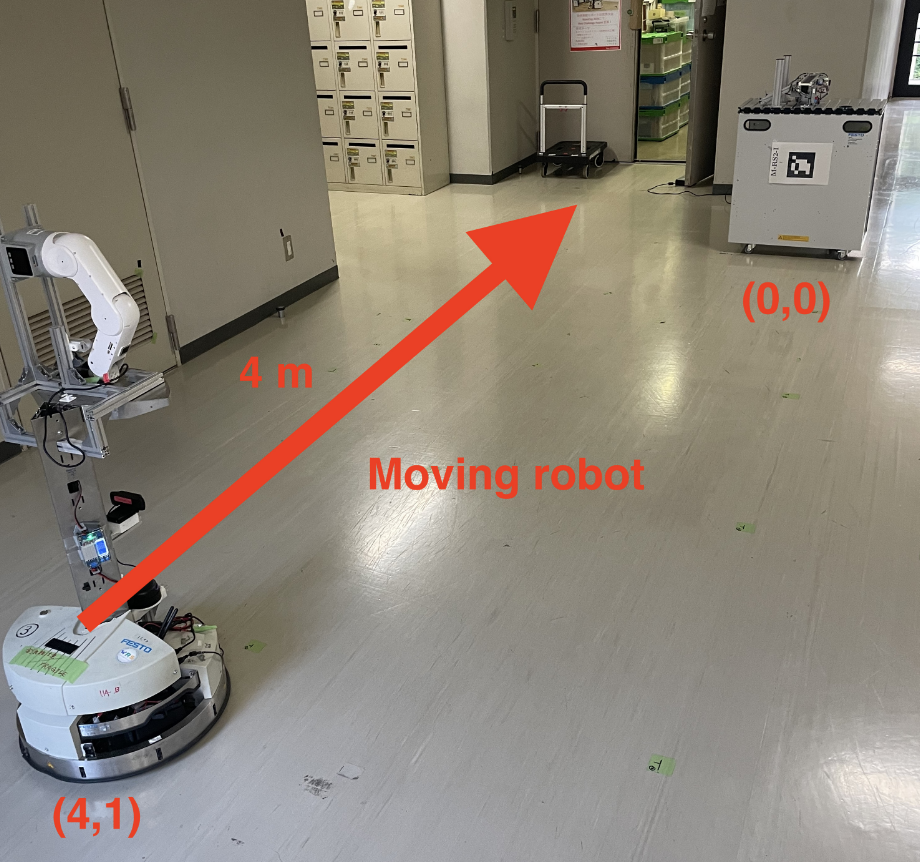
\includegraphics[width=\textwidth]{images/aruco-example-1.png}
        \caption{Robot localisation (\cite{AI-Assisted-Drone-Localization})}
        \label{fig:aruco1}
    \end{subfigure}
    \hfill
    \begin{subfigure}[b]{0.45\textwidth}
        \centering
        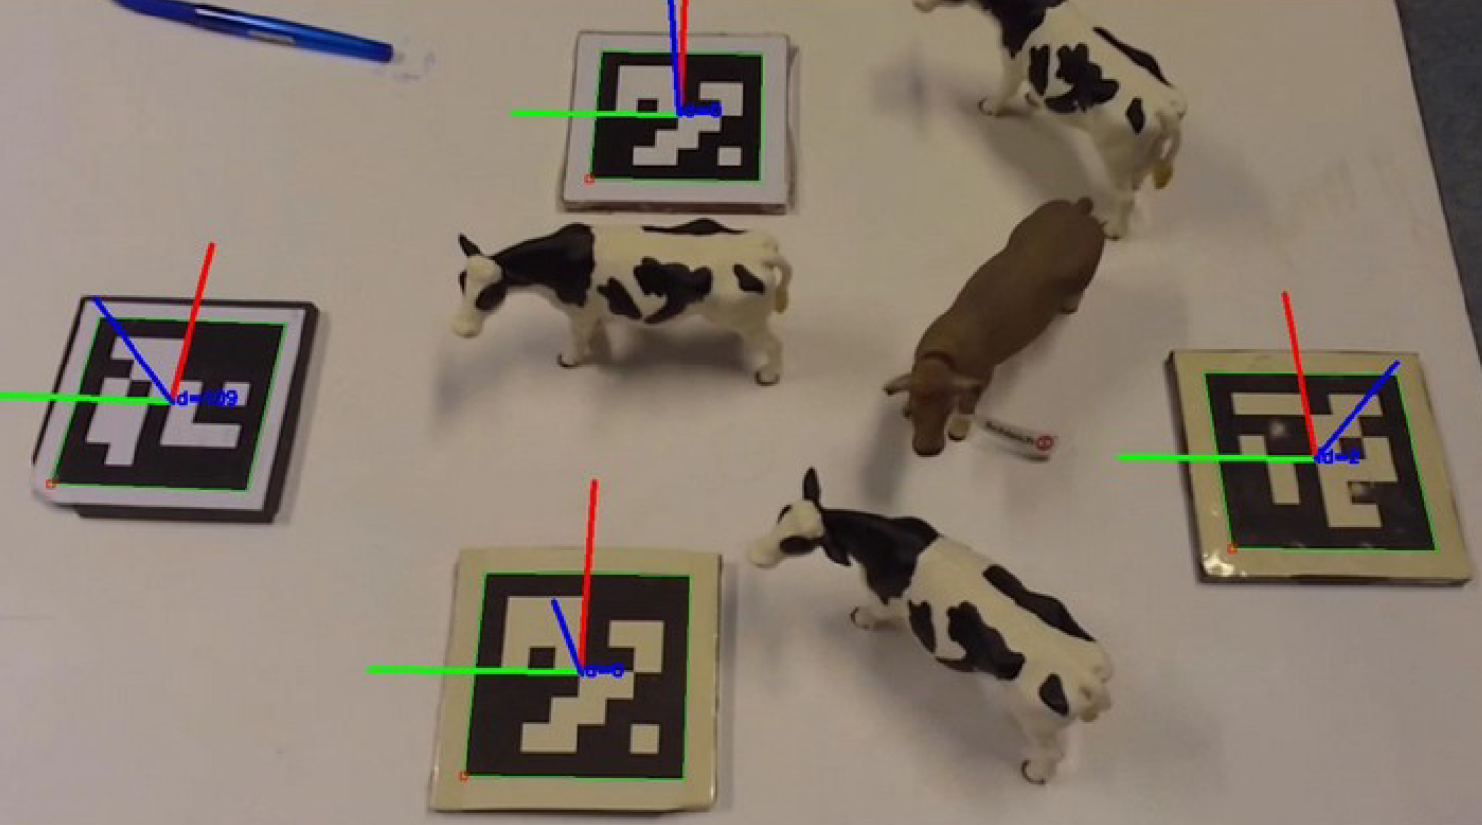
\includegraphics[width=\textwidth]{images/aruco-example-2.png}
        \caption{Drone localisation (\cite{Nakajima2024AboutAE})}
        \label{fig:aruco2}
    \end{subfigure}
    \caption{Examples of ArUco markers in different conditions}
    \label{fig:aruco_markers}
\end{figure}

However, as noted by \textcite{FiducialMarkerNoisy} and \textcite{ROMERORAMIREZ2021104094}, traditional detection methods perform well
under controlled conditions but struggle with real-world challenges such as rotation, blur, and noise. This project investigates deep
learning approaches to address these limitations. The key objectives are:

\begin{enumerate}
  \item Classifying ArUco markers under challenging conditions (blur, noise, and rotation).
  \item Detecting and tracking marker positions in noisy or distorted environments.
\end{enumerate}

\section{Classification}

\subsection{Classification Methodology}

\begin{figure}[h]
  \centering
  \begin{subfigure}[b]{0.2\textwidth}
      \centering
      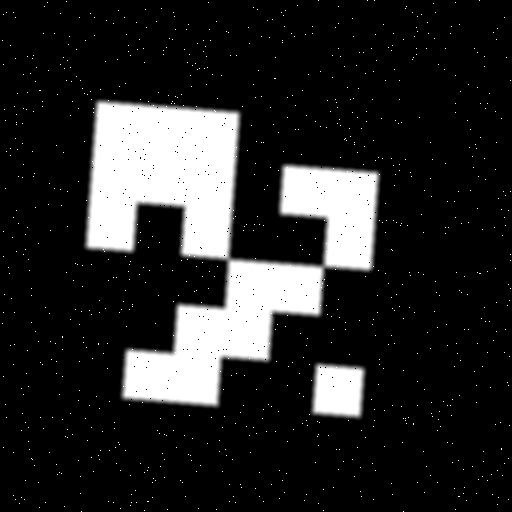
\includegraphics[width=\textwidth]{images/aruco-file3-classification-1.png}
      \caption{Class 0 (out of 100) marker example 1}
      \label{fig:class_ex1}
  \end{subfigure}
  \hfill
  \begin{subfigure}[b]{0.2\textwidth}
      \centering
      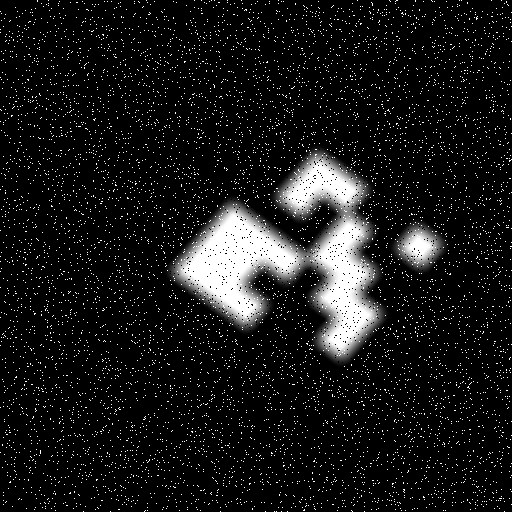
\includegraphics[width=\textwidth]{images/aruco-file3-classification-2.png}
      \caption{Class 0 (out of 100) marker example 2}
      \label{fig:class_ex2}
  \end{subfigure}
  
  \vspace{0.5cm}
  
  \begin{subfigure}[b]{0.2\textwidth}
      \centering
      
\includegraphics[width=\textwidth]{images/aruco-file3-classification-3.png}
      \caption{Class 1 (out of 100) marker example 1}
      \label{fig:class_ex3}
  \end{subfigure}
  \hfill
  \begin{subfigure}[b]{0.2\textwidth}
      \centering
      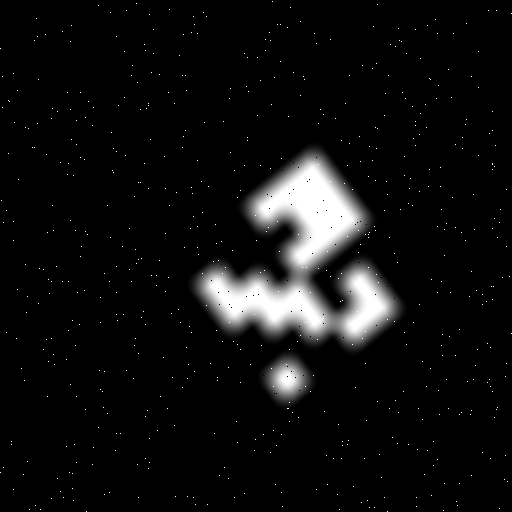
\includegraphics[width=\textwidth]{images/aruco-file3-classification-4.png}
      \caption{Class 1 (out of 100) marker example 2}
      \label{fig:class_ex4}
  \end{subfigure}
  \caption{Examples of ArUco marker classification under different conditions (from the provided dataset)}
  \label{fig:classification_examples}
\end{figure}

The classification dataset examples are visible in Figure \ref{fig:classification_examples}. The dataset contains
100 variations/classes of the ArUco marker. Developing a classification model was divided into the following steps:

\begin{enumerate}
  \item Create a data visualisation tool for datasets and results.
  \item Develop a data augmentation pipeline to expand the dataset.
  \item Prepare and implement suitable classification architectures.
  \item Design an experiment to evaluate architectures and parameters.
  \item Train and test the chosen classification model.
\end{enumerate}

\subsubsection{Data Preparation}

Firstly, a dataset browser was created to understand the data. This tool provided insight into image characteristics,
pixel distribution, and basic dataset statistics. It was also designed to visualise both datasets and results, as
demonstrated in Figure \ref{fig:data_browser_1}.

\begin{figure}[h]
  \centering
  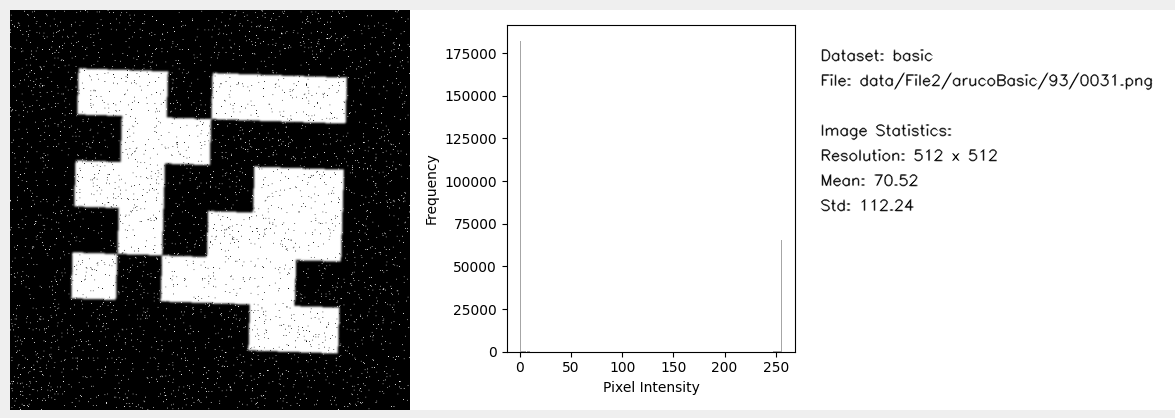
\includegraphics[width=0.45\textwidth]{images/aruco-dataset-browser-1.png}
  \caption{Dataset browser used with the File2 dataset}
  \label{fig:data_browser_1}
\end{figure}

A data augmentation pipeline was developed to generate a larger, more robust dataset. Through trial and error, augmentation
parameters were optimised to mimic the distortions observed in File3. The pipeline expanded the original dataset (100 images
in File1, each representing a different ArUco marker) to 1,000 images per class at a resolution of 512x512 pixels. Augmentations, 
including rotation, blurring, and noise, were configured via a central configuration file, allowing for flexibility without 
needing to modify the codebase. The pipeline workflow is summarised below:

\begin{figure}[H]
  \begin{algorithm}[H]
  \caption{Data Augmentation Pipeline}
  \begin{algorithmic}[1]
  \STATE List all of the images in the File1 dataset
  \WHILE{size of augmentations list $<$ target dataset size}
      \STATE Select random rotation, between 0 and 360 degrees
      \STATE Select random scaling, between 50\% and 100\% of original size
      \STATE Select random blur, between 0 and 14 sigma
      \STATE Select random noise, between 0\% and 10\% of pixels
      \STATE Append the set of augmentations to the list
    \ENDWHILE
  \FOR{each image in File1}
      \STATE Create folder named after the image's number (0-99)
      \STATE Read the raw image
      \FOR{each set in the list of augmentations}
        \STATE Apply the augmentations to the image
        \STATE Save the augmented image to the new folder
      \ENDFOR
    \ENDFOR
  \end{algorithmic}
  \end{algorithm}
  \caption{Classification training workflow}
  \end{figure}

\subsubsection{Network Architectures}

Several classification architectures were implemented using PyTorch, starting with a basic convolutional neural network (CNN)
to establish baseline performance. Following this, pre-trained and non-pre-trained variants of AlexNet were tested. ResNet18
and GoogLeNet were also evaluated, leveraging PyTorch documentation and guidelines \textcite{pytorch_models}. The codebase was
modular, allowing seamless integration of new models into experiments.

The following architectures were selected for initial experimentation:

\begin{itemize}
    \item \textbf{MinimalCNN}: A lightweight custom architecture with:
    \begin{itemize}
        \item Three convolutional blocks (32$\rightarrow$64$\rightarrow$128 features)
        \item Batch normalisation and dropout for regularisation
        \item Global average pooling for dimension reduction
    \end{itemize}
    
    \item \textbf{AlexNet Variants}:
    \begin{itemize}
        \item Clean implementation without pre-training
        \item Version with pre-trained features
    \end{itemize}
    
    \item \textbf{ResNet18}: Pre-trained implementation
    \item \textbf{GoogLeNet}: Pre-trained implementation
\end{itemize}

\subsubsection{Training Configuration}

The experiments tested combinations of the above architectures with varied parameters:

\begin{itemize}
  \item \textbf{Datasets}: File3 (100 images per class, significant distortions).
  \item \textbf{Models}: MinimalCNN, AlexNet (clean), AlexNet, ResNet18, GoogLeNet.
  \item \textbf{Batch Sizes}: 32, 64.
  \item \textbf{Training Transformations}: None, random rotations, and combinations of rotations, blur, and noise.
\end{itemize}

This resulted in 30 parameter/model combinations, trained over nearly 8 hours on a single GPU. Customisation required
minimal effort, achieved via a central configuration file. Adjustments could be made to also trial and compare other combinations with
datasets, batch sizes, learning rates, transformations, and models, although most of these were not tested due to GPU memory constraints.
The selected learning rate and training duration were chosen during the initial experiments throught the development, this can be seen 
in some of the past GitHub commits.

\begin{itemize}
    \item \textbf{Loss Function}: Cross-entropy
    \item \textbf{Optimizer}: Adam with learning rate 3e-4
    \item \textbf{Training Duration}: 50 epochs with early stopping at 96\% training accuracy 
\end{itemize}

Once training was complete, results were plotted and analysed. Full results are detailed in the appendices and results directory.
The final classification model was trained on the custom dataset with the following optimised parameters:

\begin{itemize}
  \item \textbf{Datasets}: Custom dataset (1000 images per class)
  \item \textbf{Model}: GoogLeNet
  \item \textbf{Batch Sizes}: 32
  \item \textbf{Additional Random Training Transformations}: None
\end{itemize}

\subsubsection{Method Implementation}

The experiment implementation followed this algorithmic workflow:

\begin{figure}[H]
\begin{algorithm}[H]
\caption{Classification Experiment Pipeline}
\begin{algorithmic}[1]
\STATE Load configuration for dataset, model, batch size, and transformations
\FOR{each combination in configurations}
    \STATE Load dataset
    \STATE Setup results directory
    \STATE Initialise model and transforms
    \STATE Create data loaders
    \STATE Initialise loss function, optimiser
    \STATE Train and validate model for number of epochs
    \STATE Plot the training progress
    \STATE Run evaluation on test set
    \STATE Plot classification metrics
    \STATE Save all results
\ENDFOR
\end{algorithmic}
\end{algorithm}
\caption{Classification experiment workflow}
\end{figure}

The model training loop is shown below:

\begin{figure}[H]
\begin{algorithm}[H]
\caption{Classification Training and Validation Pipeline}
\begin{algorithmic}[1]
\FOR{each epoch in total number of epochs}
    \STATE Set model to train mode
    \FOR{each batch in train loader}
        \STATE Reset gradients
        \STATE Forward pass through network
        \STATE Calculate cross-entropy loss
        \STATE Backpropagate and update weights
        \STATE Add loss and accuracy to totals
    \ENDFOR
    \STATE Calculate average training loss and accuracy
    \STATE Set model to evaluation mode
    \FOR{each batch in validation loader}
        \STATE Forward pass through network
        \STATE Calculate cross-entropy loss
        \STATE Add loss and accuracy to totals
    \ENDFOR
    \STATE Calculate average validation loss and accuracy
    \STATE Save model if the best validation accuracy was achieved
    \STATE Check for early stopping criteria
\ENDFOR
\end{algorithmic}
\end{algorithm}
\caption{Classification training workflow}
\end{figure}

After training, the model was tested using the original datasets (File2 and File3) to evaluate its
generalisation capabilities without seeing the originally provided data. Test-only data loaders were
created for this purpose, and the model performance on these datasets was separately recorded.

\subsection{Classification Results}

The classification experiments were conducted in two phases. Initially, multiple architectures and configurations were tested on the
File3 dataset to determine the optimal approach. Subsequently, the best performing configuration was trained on a custom dataset and
was evaluated against separately File2 and File3 datasets.

\subsubsection{Initial Experiments}

Various architectures with different batch sizes and data augmentation strategies were explored. Each configuration was tested on
1000 samples from File3, with the following (best of) results. The full results of each combination can be seen in the repository.

\begin{itemize}
    \item \textbf{MinimalCNN}:
        \begin{itemize}
            \item Batch size 32, full (training time) augmentation: 5.20\% accuracy (F1: 3.62\%)
        \end{itemize}

    \item \textbf{AlexNet (Clean Implementation)}:
        \begin{itemize}
            \item Batch size 64, rotation (training time) augmentation: 98.60\% accuracy (F1: 98.51\%)
        \end{itemize}
    
    \item \textbf{AlexNet (Pre-trained)}:
        \begin{itemize}
            \item Batch size 64, full (training time) augmentation: 73.70\% accuracy (F1: 72.15\%)
        \end{itemize}
    
    \item \textbf{ResNet18}:
        \begin{itemize}
            \item Batch size 32, no (training time) augmentation: 100.00\% accuracy (F1: 100.00\%)
        \end{itemize}
    
    \item \textbf{GoogLeNet}:
        \begin{itemize}
            \item Batch size 32, no (training time) augmentation: 99.90\% accuracy (F1: 99.87\%)
        \end{itemize}
\end{itemize}

The experiment results are shown in the figure \ref{fig:training_progress}.

\begin{figure}[h]
    \centering
    \begin{subfigure}[b]{0.45\textwidth}
      \centering
      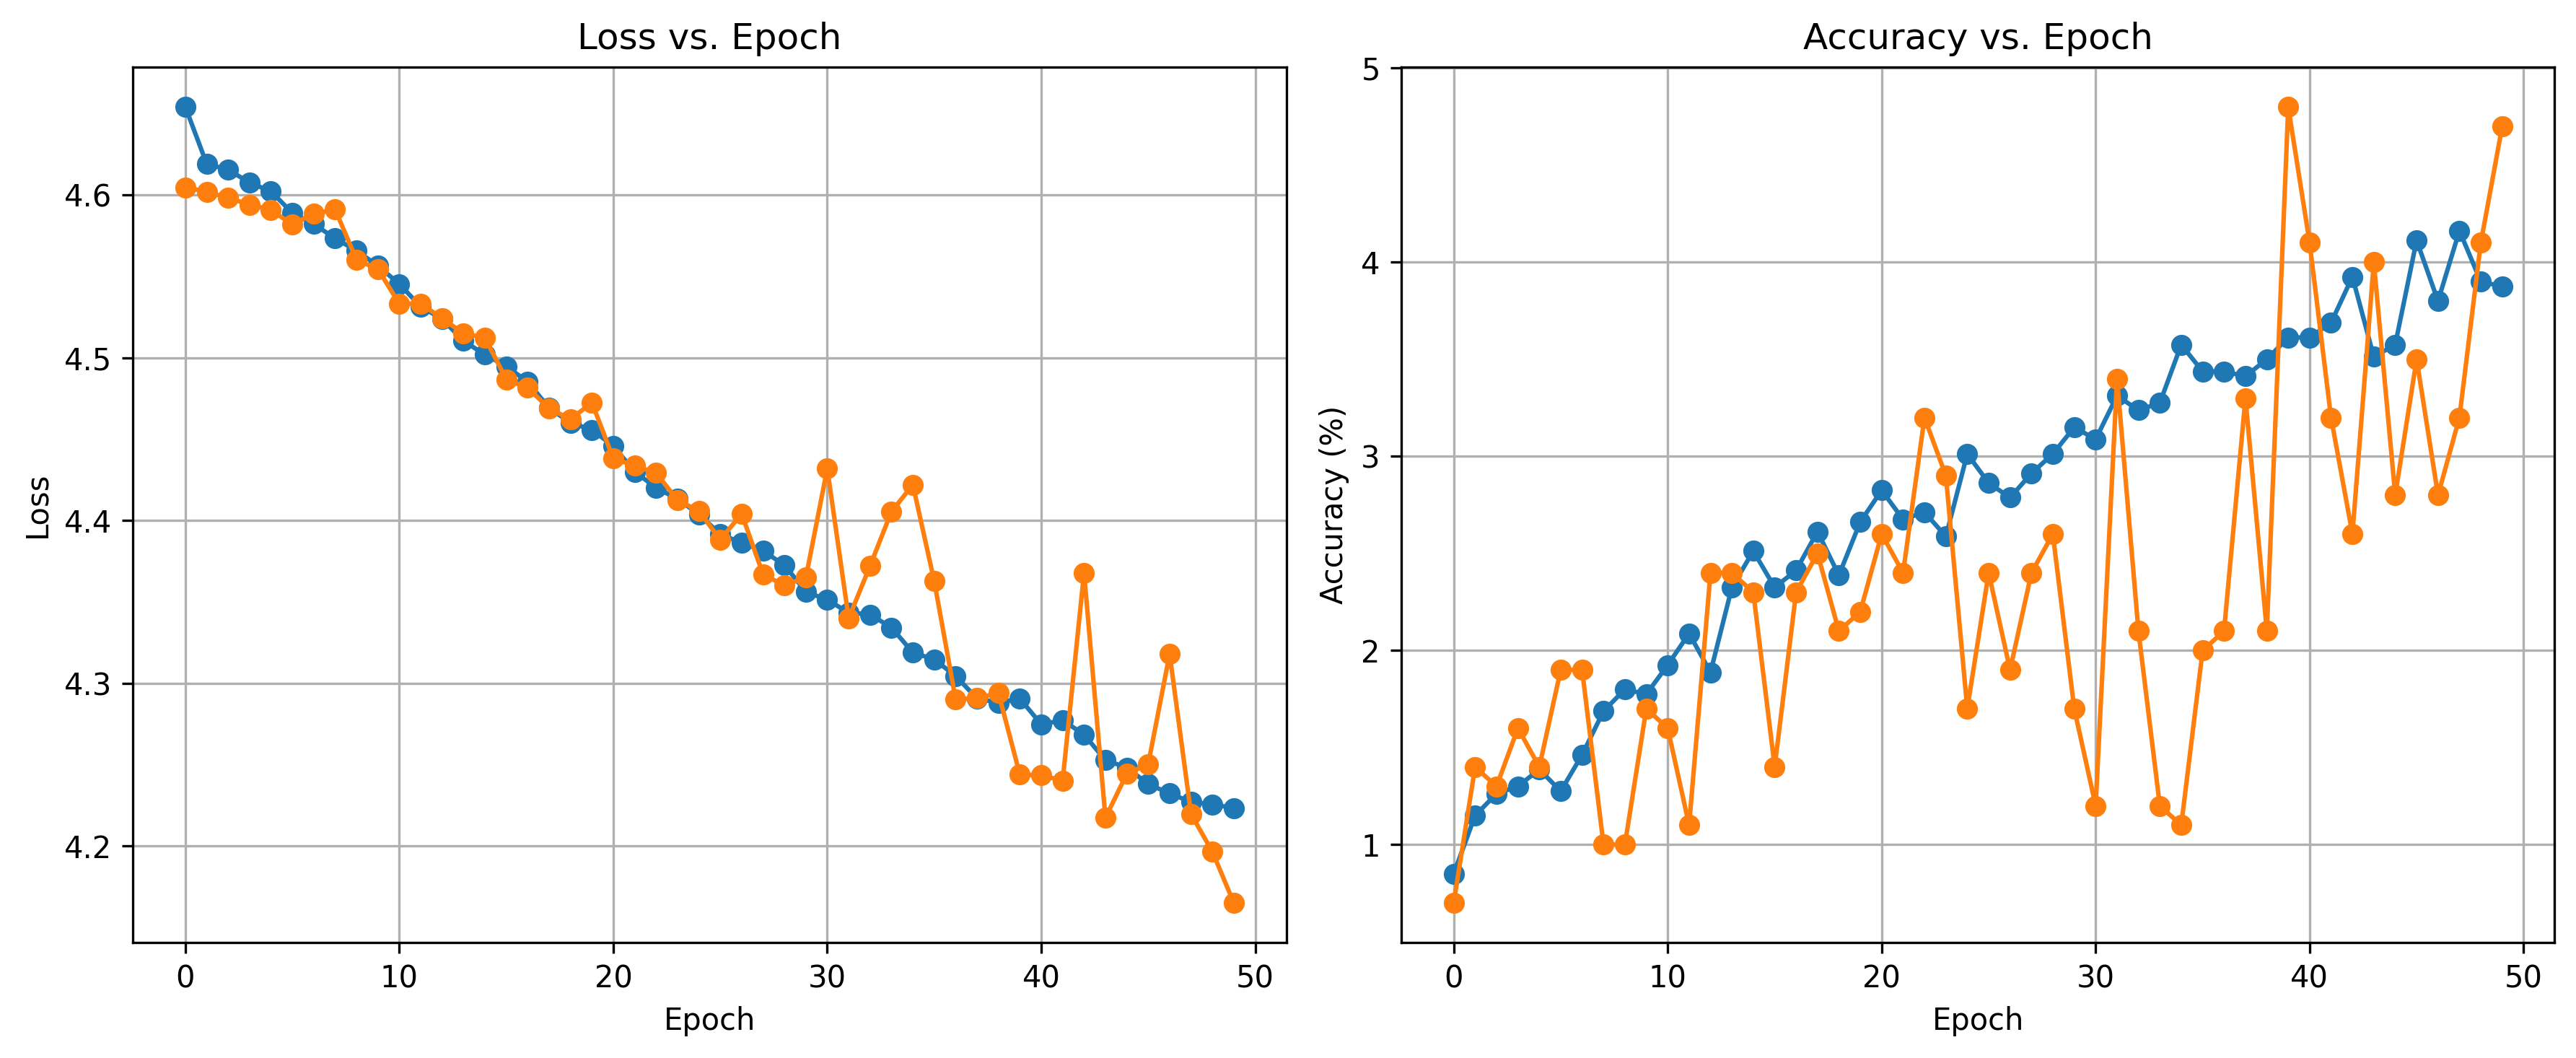
\includegraphics[width=\textwidth]{images/training_progress_MinimalCNN.png}
      \caption{MinimalCNN training progress}
      \label{fig:progress_minimalcnn}
    \end{subfigure}
    \hfill
    \begin{subfigure}[b]{0.45\textwidth}
      \centering
      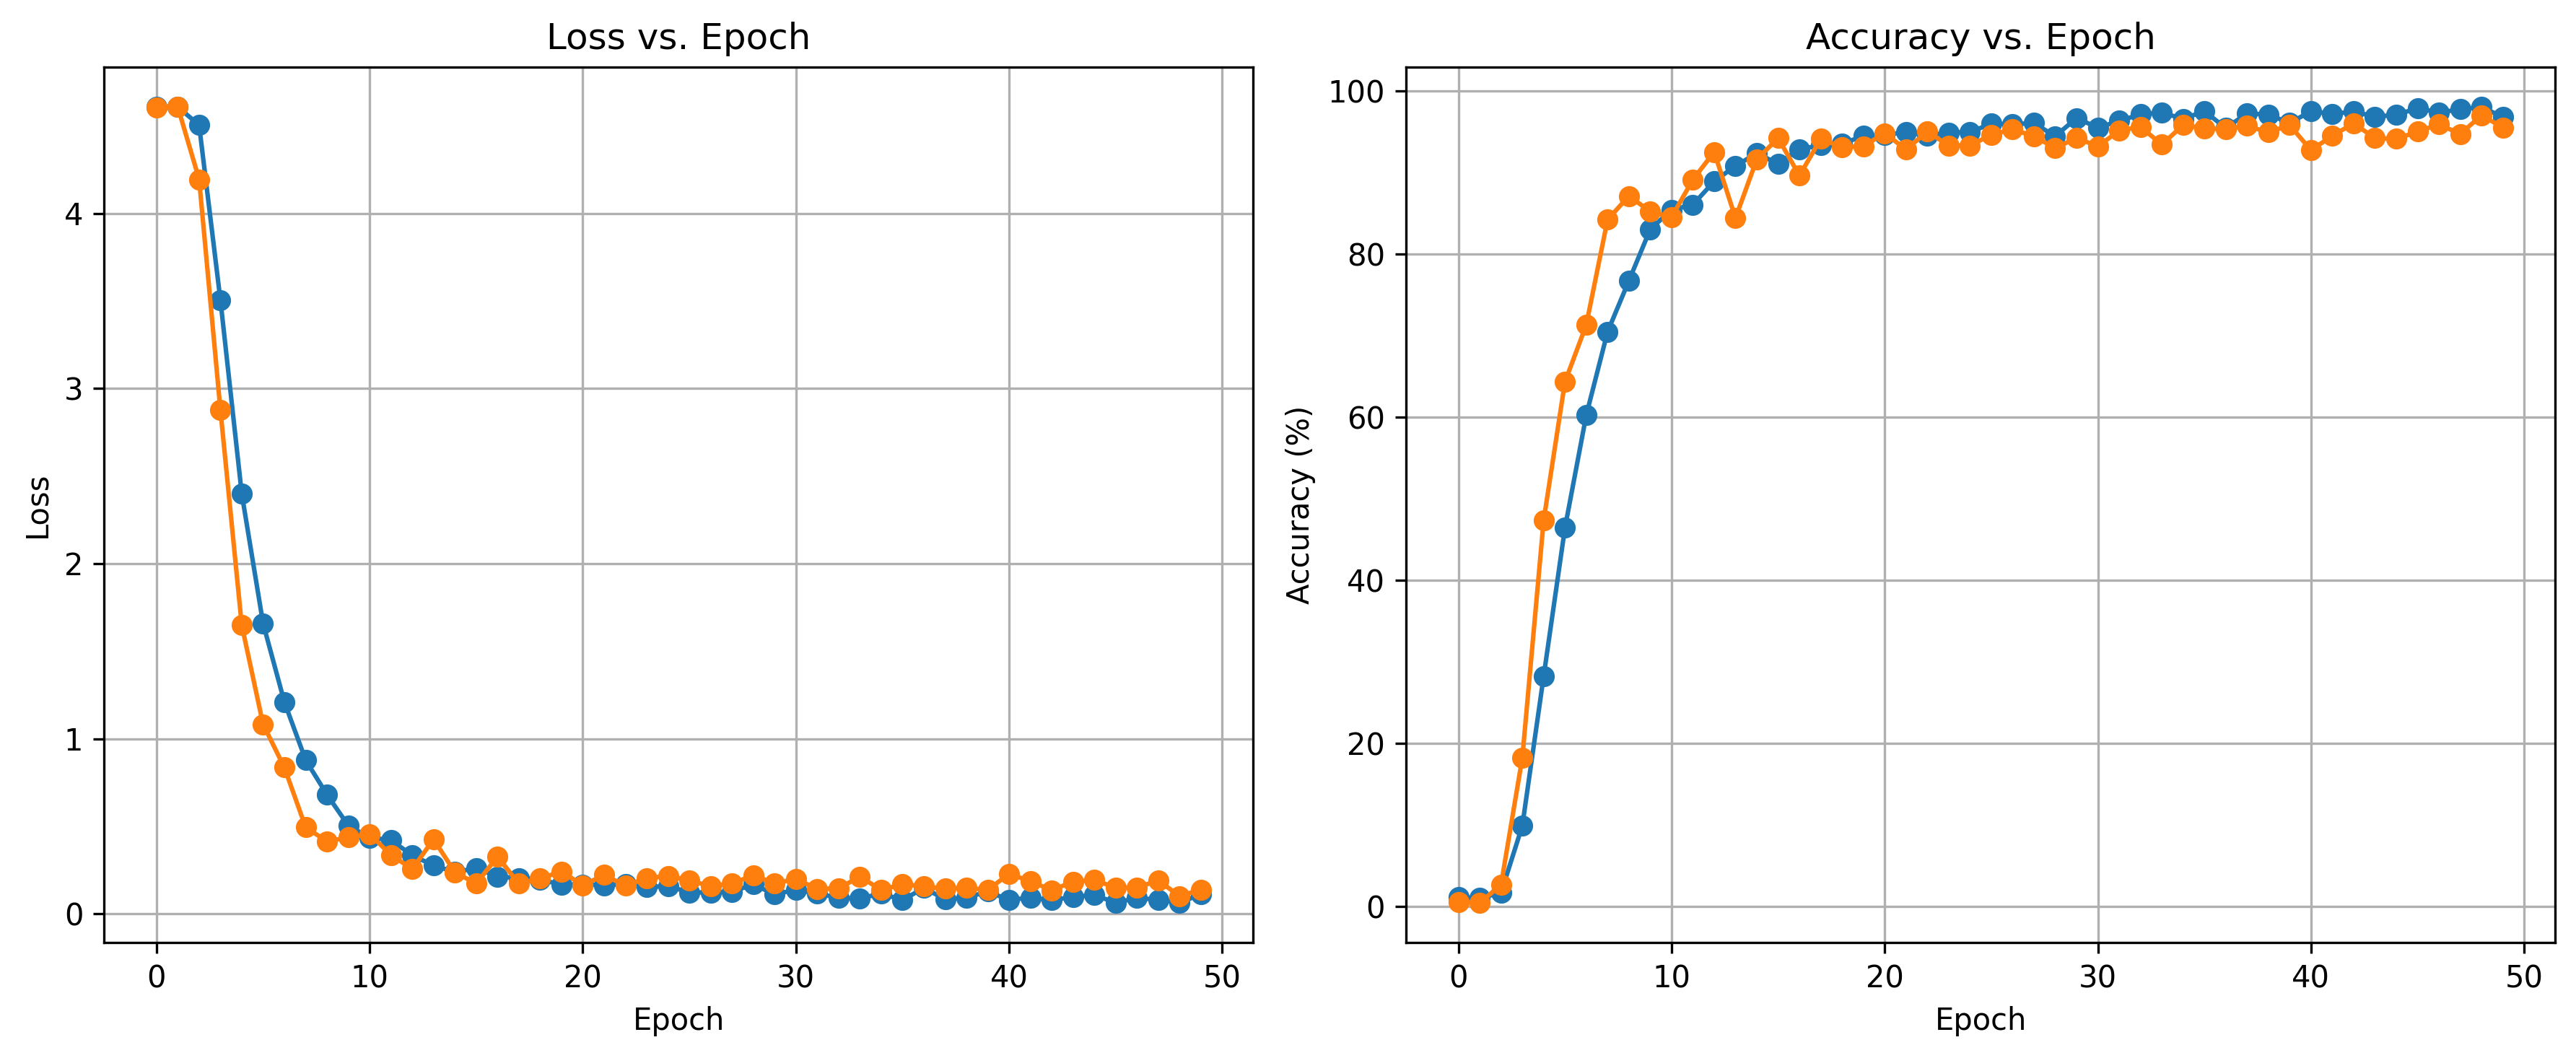
\includegraphics[width=\textwidth]{images/training_progress_AlexNet_clean.png}
      \caption{AlexNet (clean) training progress}
      \label{fig:progress_alexnet_clean}
    \end{subfigure}    
    \vspace{0.5cm}
    \begin{subfigure}[b]{0.45\textwidth}
      \centering
      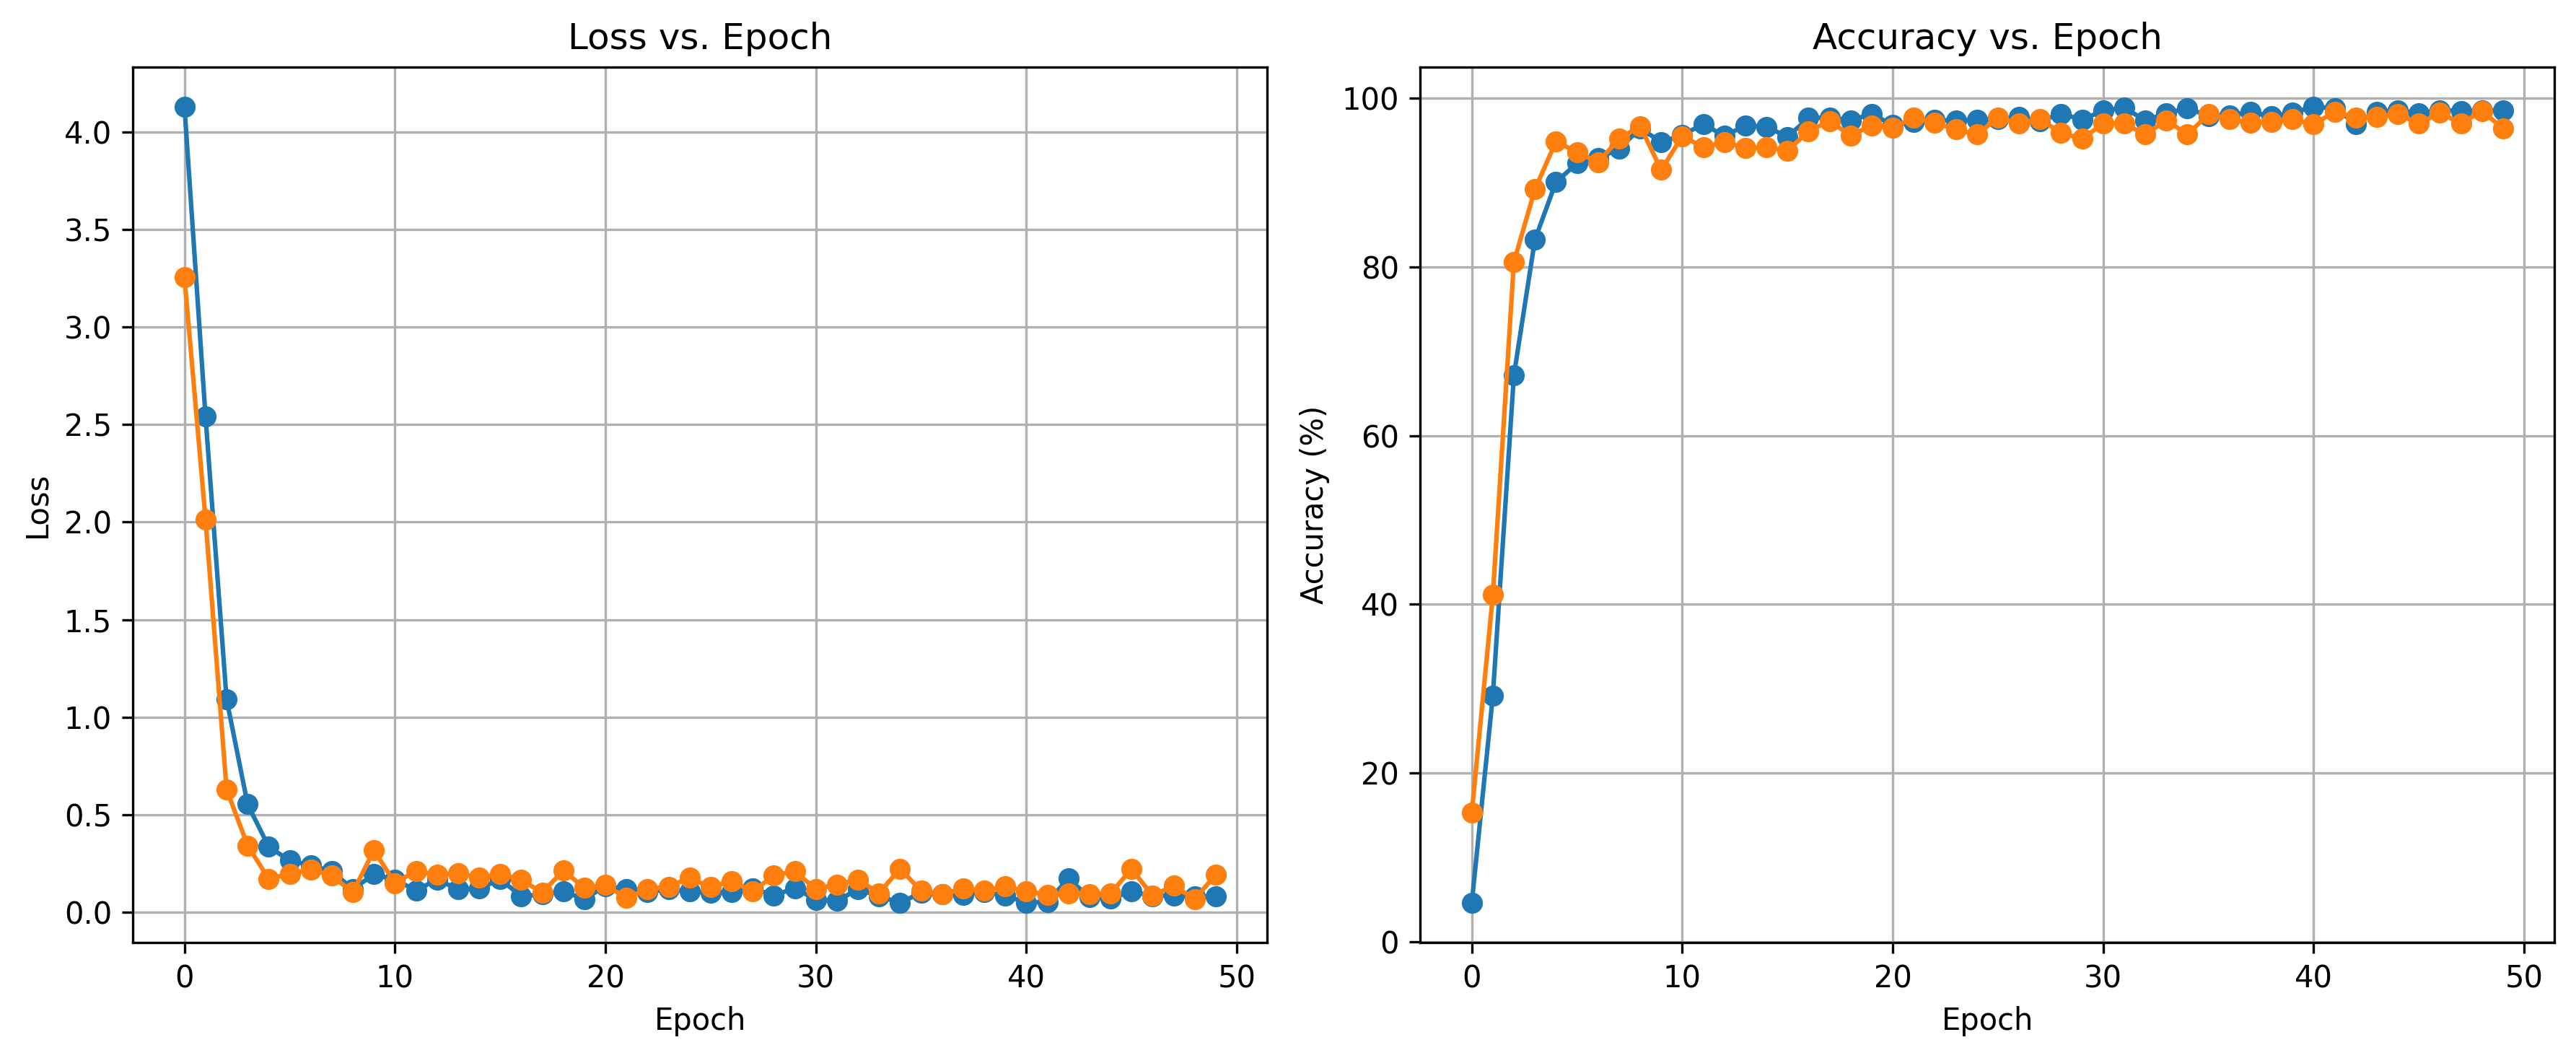
\includegraphics[width=\textwidth]{images/training_progress_AlexNet.png}
      \caption{AlexNet (pre-trained) training progress}
      \label{fig:progress_alexnet}
    \end{subfigure}
    \hfill
    \begin{subfigure}[b]{0.45\textwidth}
        \centering
        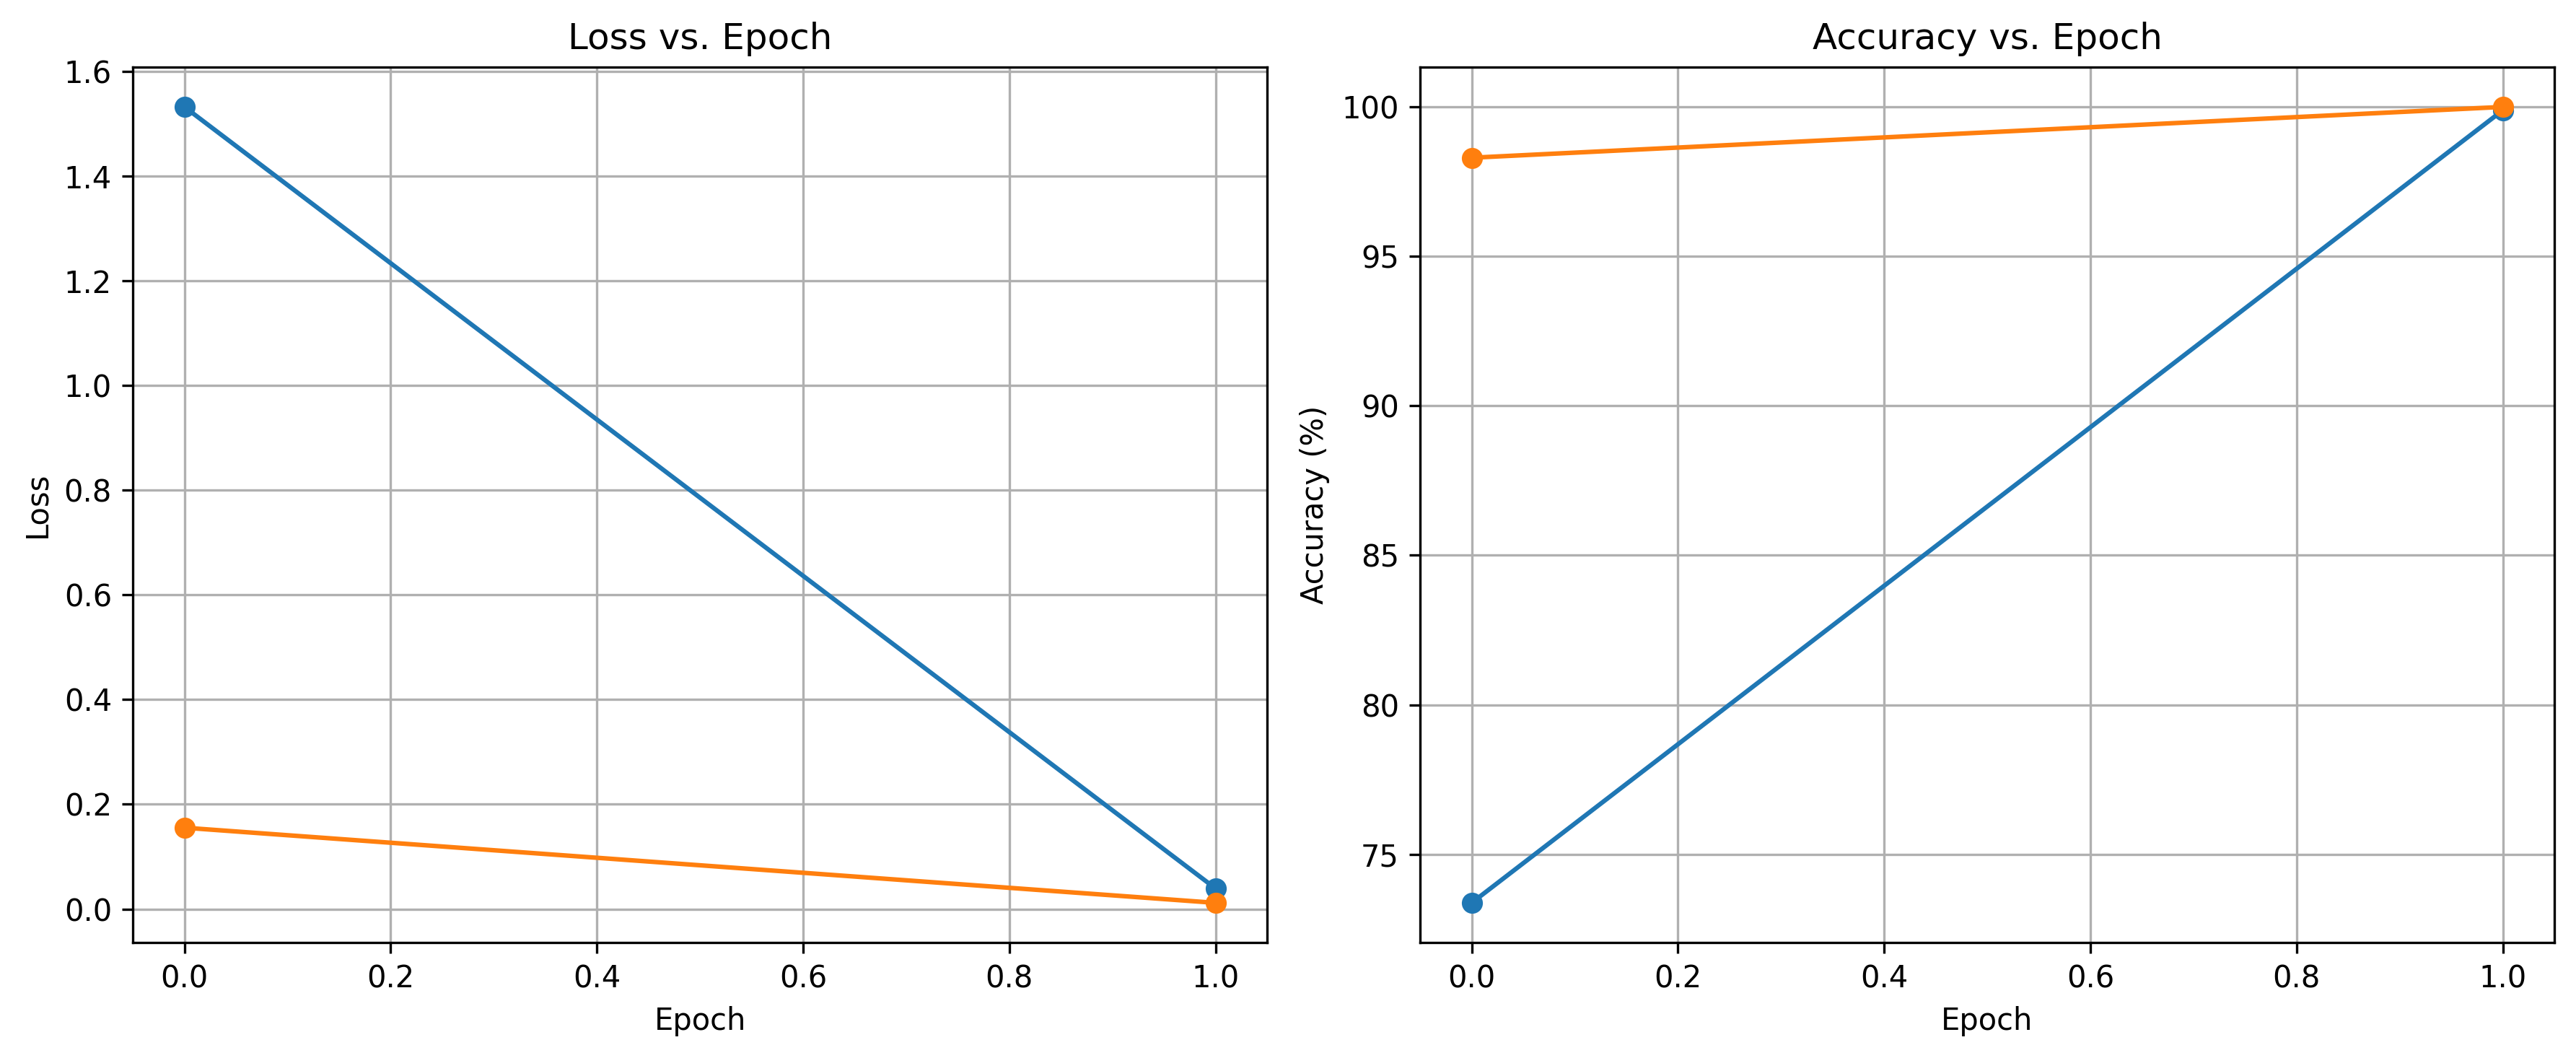
\includegraphics[width=\textwidth]{images/training_progress_ResNet.png}
        \caption{ResNet18 training progress}
        \label{fig:progress_resnet}
    \end{subfigure}
    \caption{Training progress for different model architectures showing training and validation accuracy over epochs (orange plot is validation accuracy,
    blue is training accuracy)}
    \label{fig:training_progress}
\end{figure}

The progress of models trained with a batch size of 32 and no data augmentation for comparability is shown in all training plots. The
minimal CNN was observed to behave as anticipated, although better performance would likely be achieved with additional epochs. 

AlexNet with no pre-trained weights was observed to perform very well, though it converged more slowly than its pre-trained counterpart.
ResNet18 and GoogLeNet were found to have performed almost perfectly and were noticeably better without additional training transforms.
Out of GoogLeNet and ResNet18, the ResNet plot is shown, as the results were essentially identical. Early stopping was triggered for both models once 99\% 
validation accuracy was reached.

For further insights, training logs and detailed analysis are provided in the appendices, which also contain additional plots, results, and data.

\subsubsection{Final Model Performance}

Based on the previous findings, GoogLeNet was chosen as the final model because of its consistent performance across different parameter
settings. Training was conducted on FileCustom1, a synthetic dataset created to approximate conditions in Files 2 and 3. The training set
size was thereby increased from 9,000 to 95,000 samples.

The following results were provided by the final evaluation:

\begin{itemize}
    \item \textbf{Training Evaluation} (2,500 samples):
        \begin{itemize}
            \item Accuracy: 100.00\%
            \item Precision: 100.00\%
            \item Recall: 100.00\%
            \item F1-score: 100.00\%
        \end{itemize}
    \item \textbf{File2 Evaluation} (10,000 samples):
        \begin{itemize}
            \item Accuracy: 100.00\%
            \item Precision: 100.00\%
            \item Recall: 100.00\%
            \item F1-score: 100.00\%
        \end{itemize}
    \item \textbf{File3 Evaluation} (10,000 samples):
        \begin{itemize}
            \item Accuracy: 97.48\%
            \item Precision: 97.68\%
            \item Recall: 97.48\%
            \item F1-score: 97.51\%
        \end{itemize}
\end{itemize}

Near-perfect performance (as shown in Figure \ref{fig:final_analysis}) under various distortion conditions is indicated by these results.
Perfect scores were achieved on File2, suggesting that weak distortions were handled effectively, whereas a strong outcome on File3 (only
252 misclassifications out of 10,000 samples) demonstrates good resilience in more challenging scenarios. Based on the per-class accuracy,
precision, and recall plots, marker 33 was identified as the most difficult class, as its precision was lowest, while markers 14 and 39
were missed most often because of the lowest recall. A clearer depiction of these findings is provided by the confusion matrix in the appendices.

\begin{figure}[h]
    \centering
    \begin{subfigure}[b]{0.45\textwidth}
        \centering
        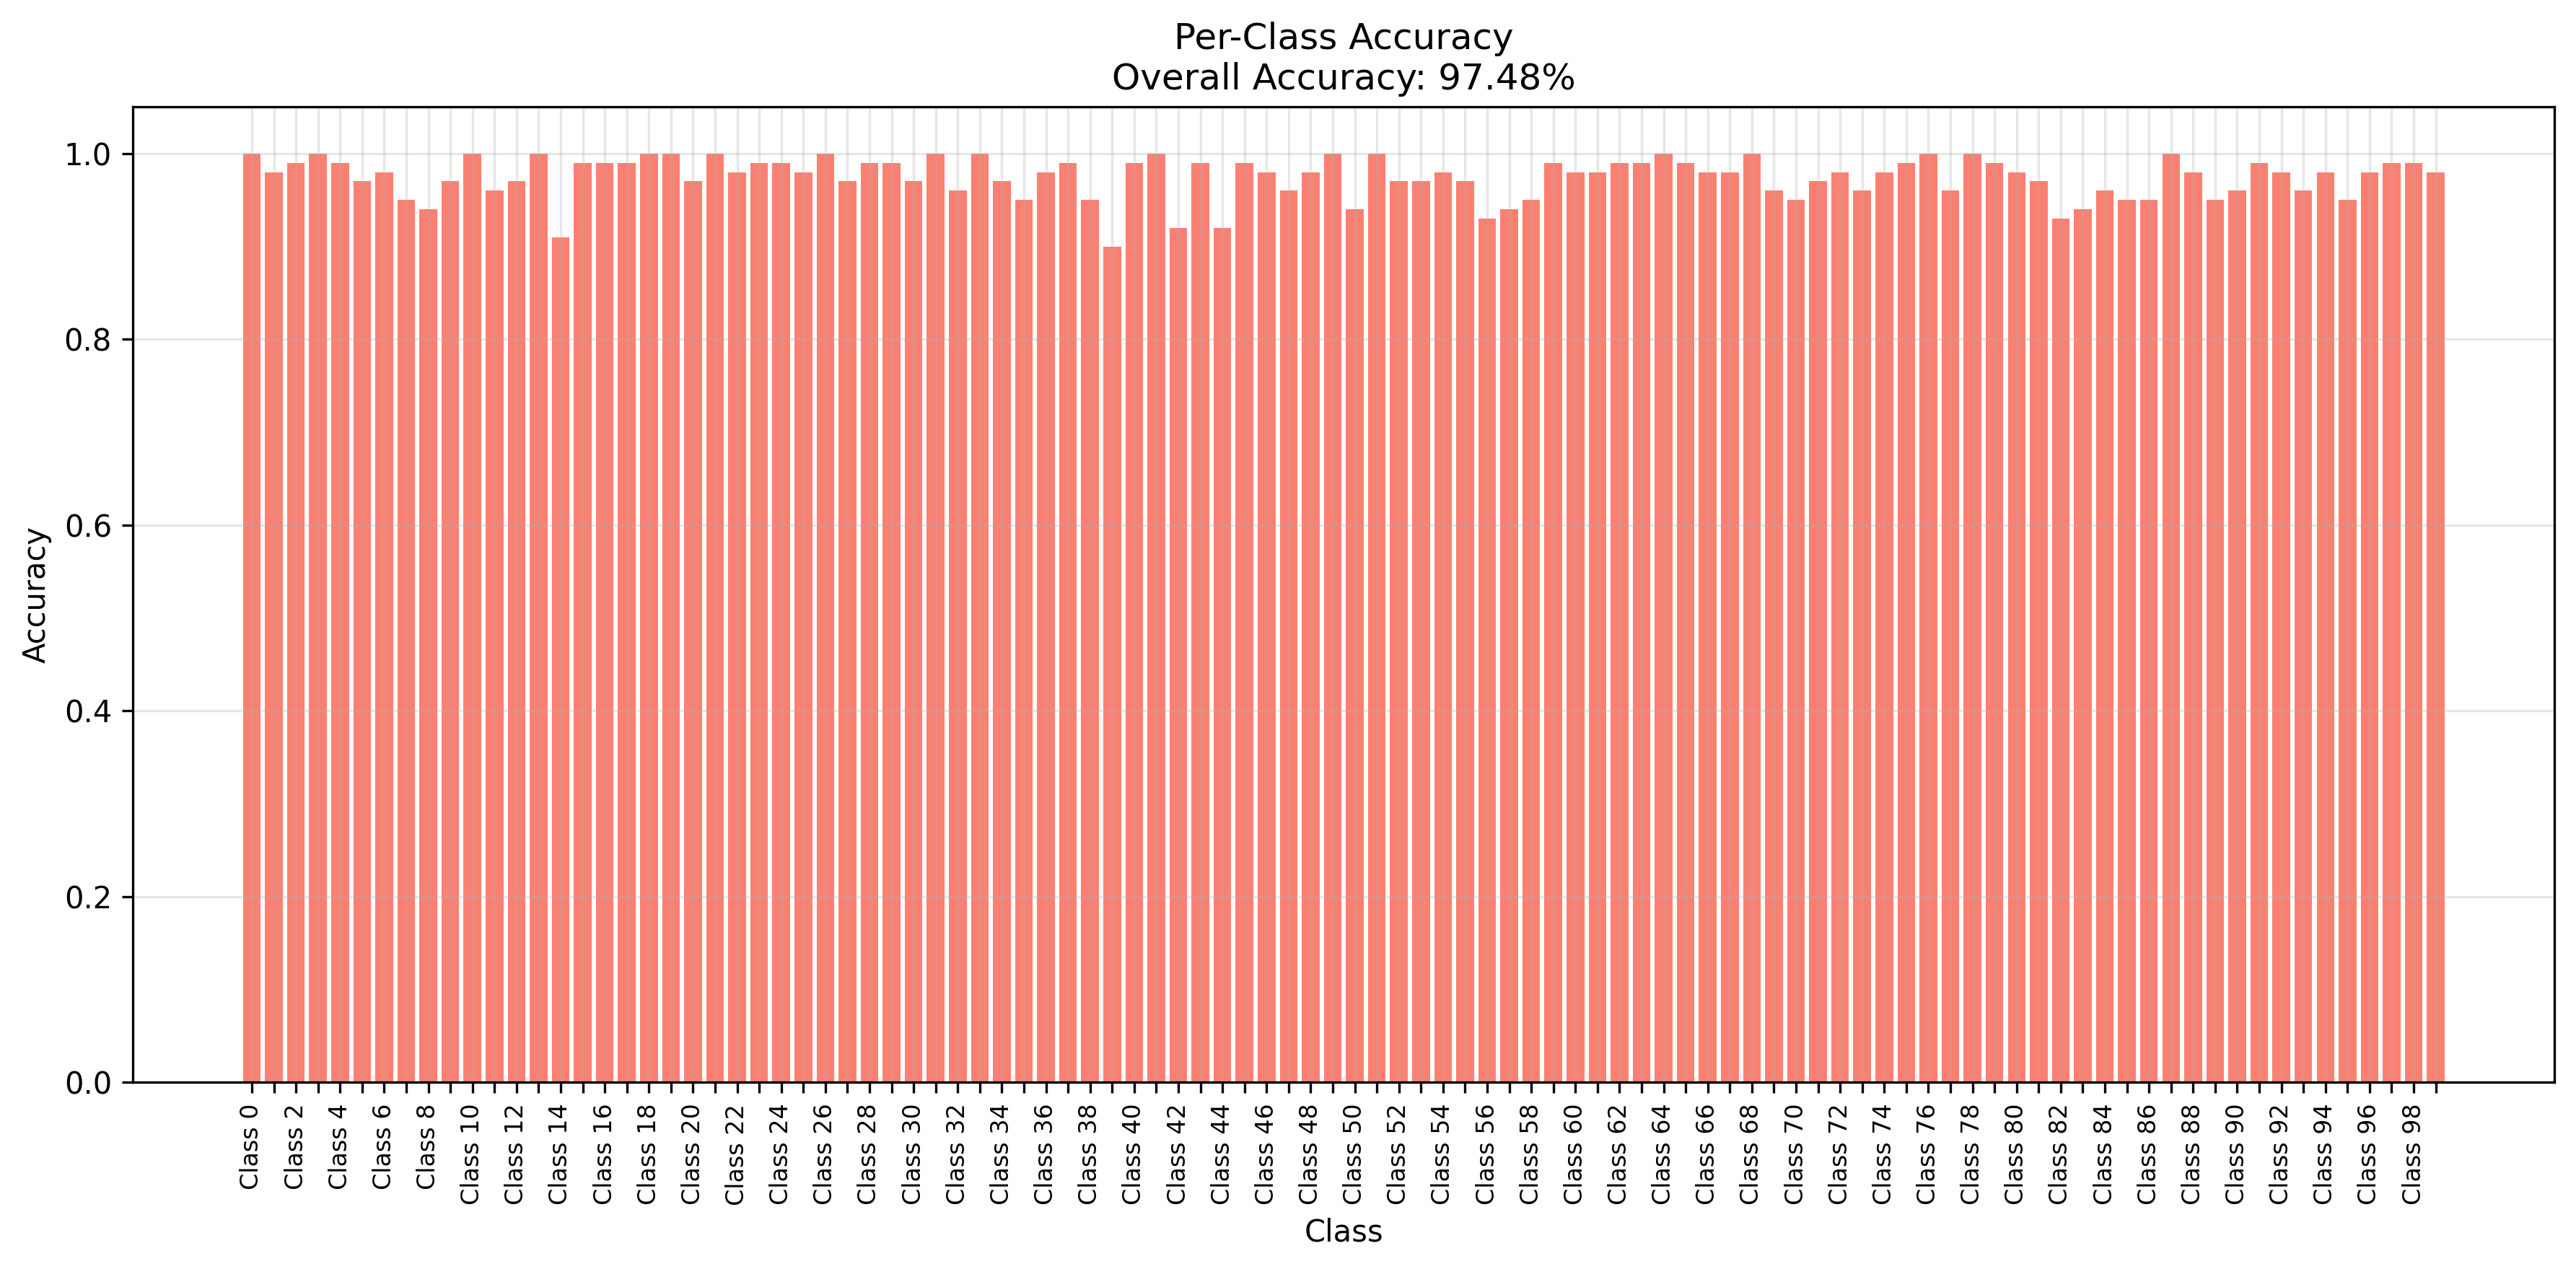
\includegraphics[width=\textwidth]{images/File3_final_analysis_accuracy.png}
        \caption{Per-class accuracy analysis}
        \label{fig:final_accuracy}
    \end{subfigure}
    \hfill
    \begin{subfigure}[b]{0.45\textwidth}
        \centering
        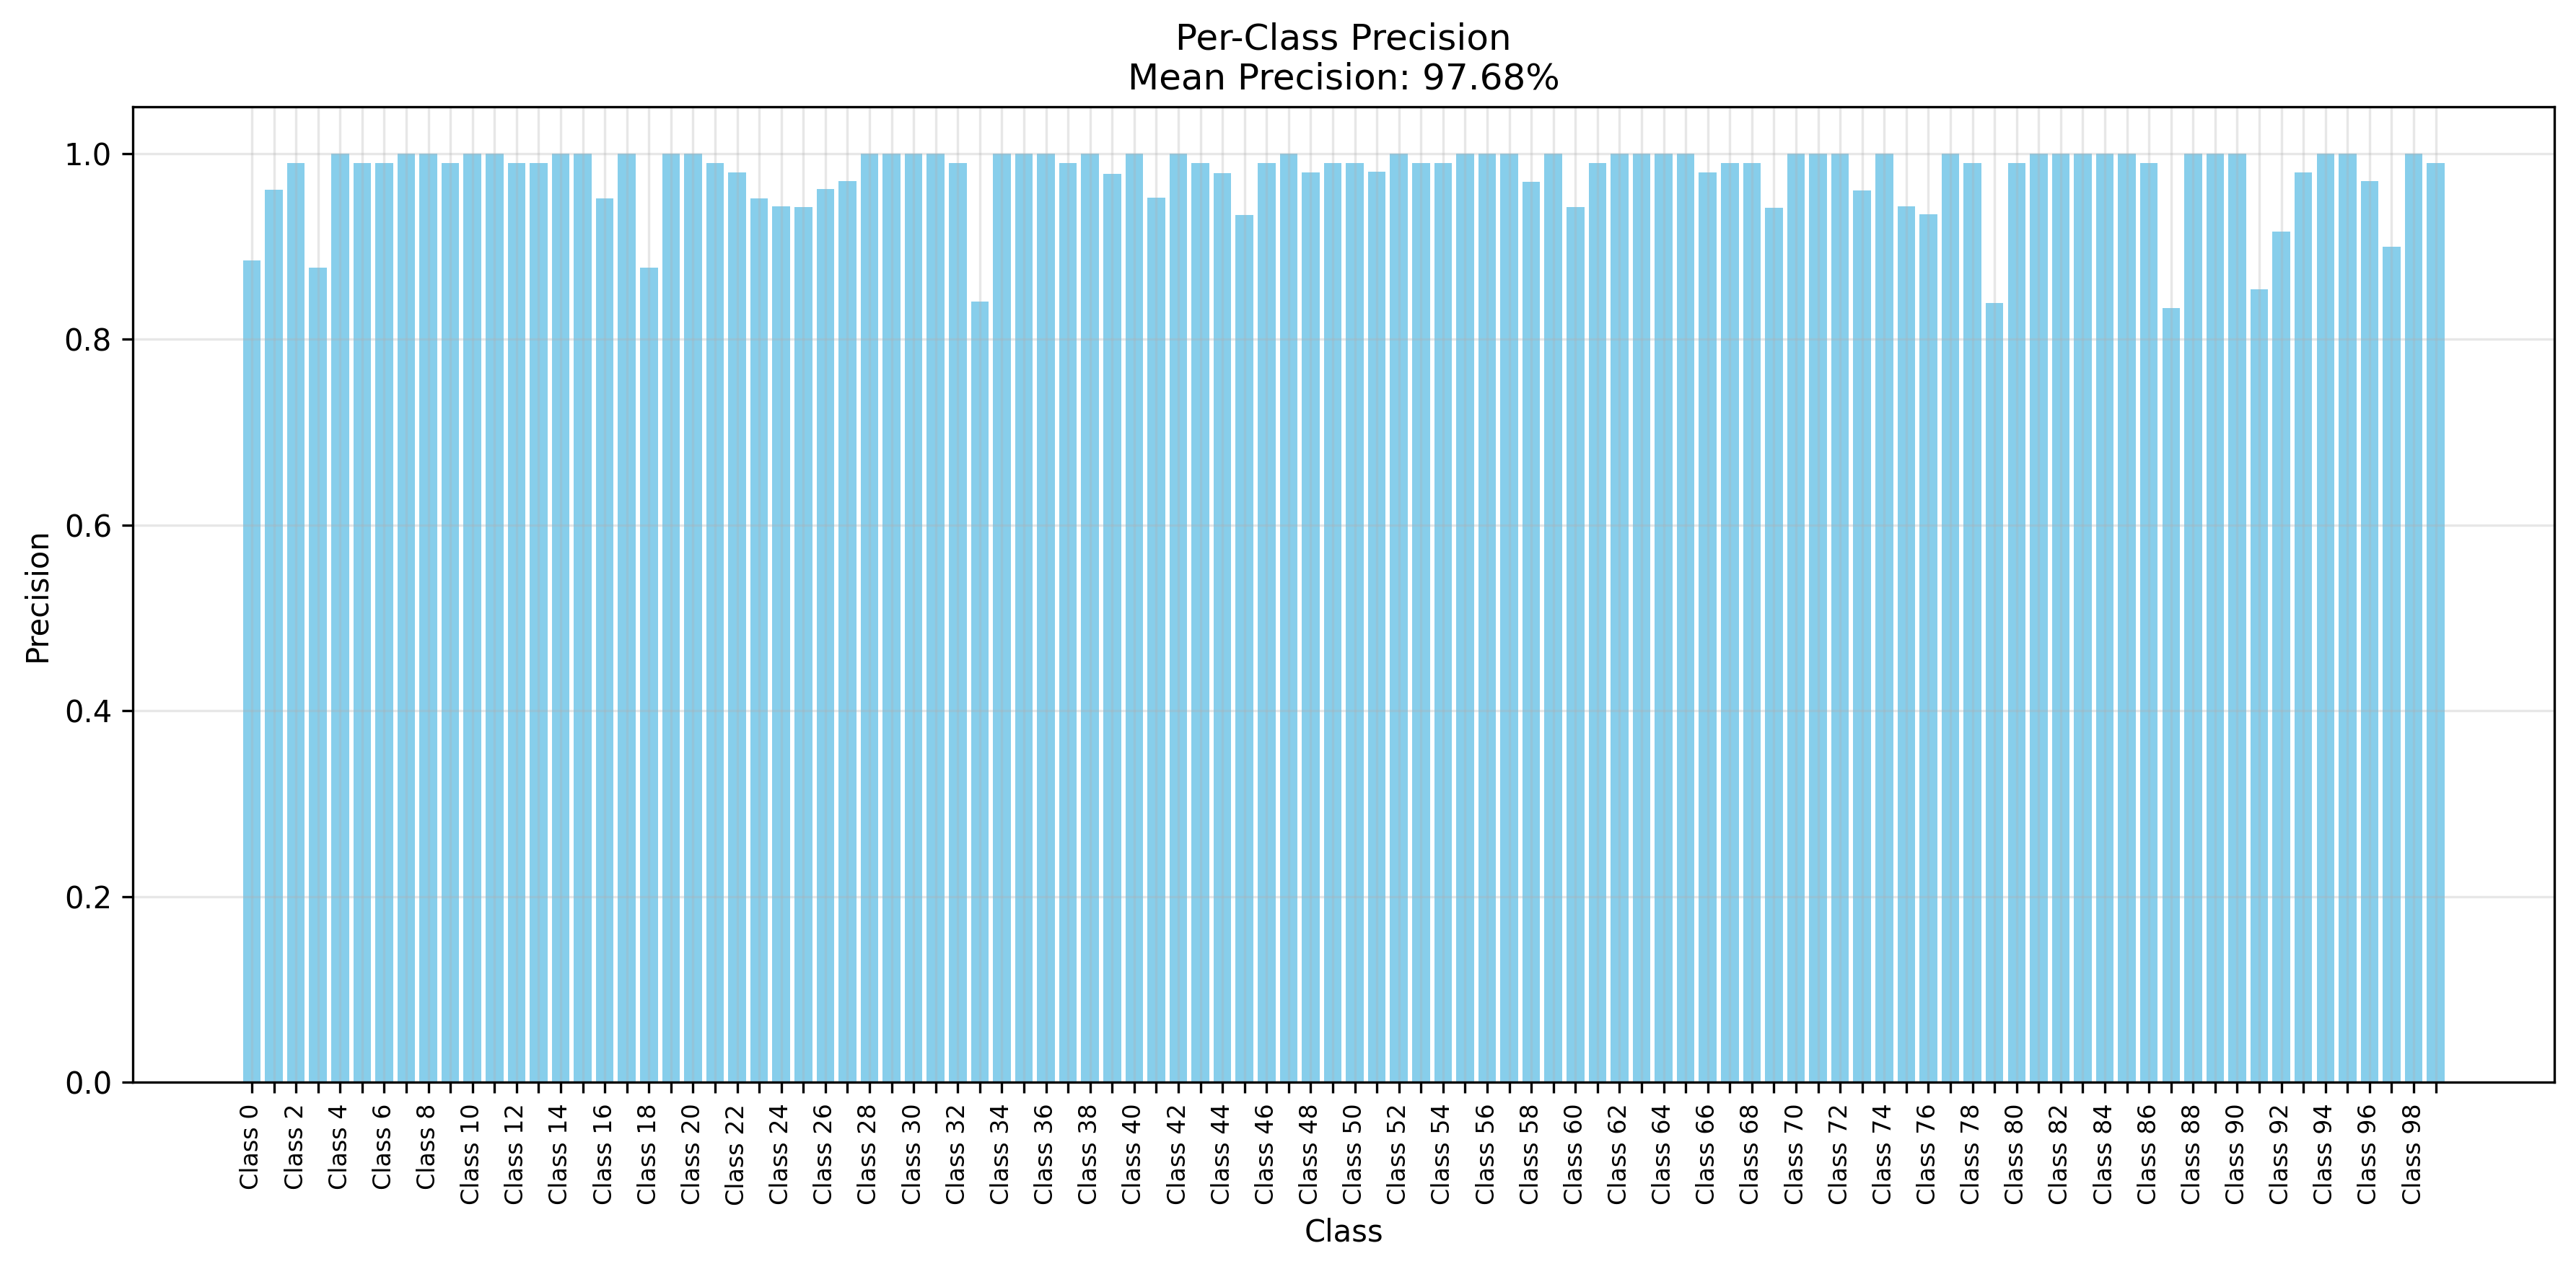
\includegraphics[width=\textwidth]{images/File3_final_analysis_precision.png}
        \caption{Per-class precision analysis}
        \label{fig:final_precision}
    \end{subfigure}
    
    \vspace{0.5cm}
    
    \begin{subfigure}[b]{0.45\textwidth}
        \centering
        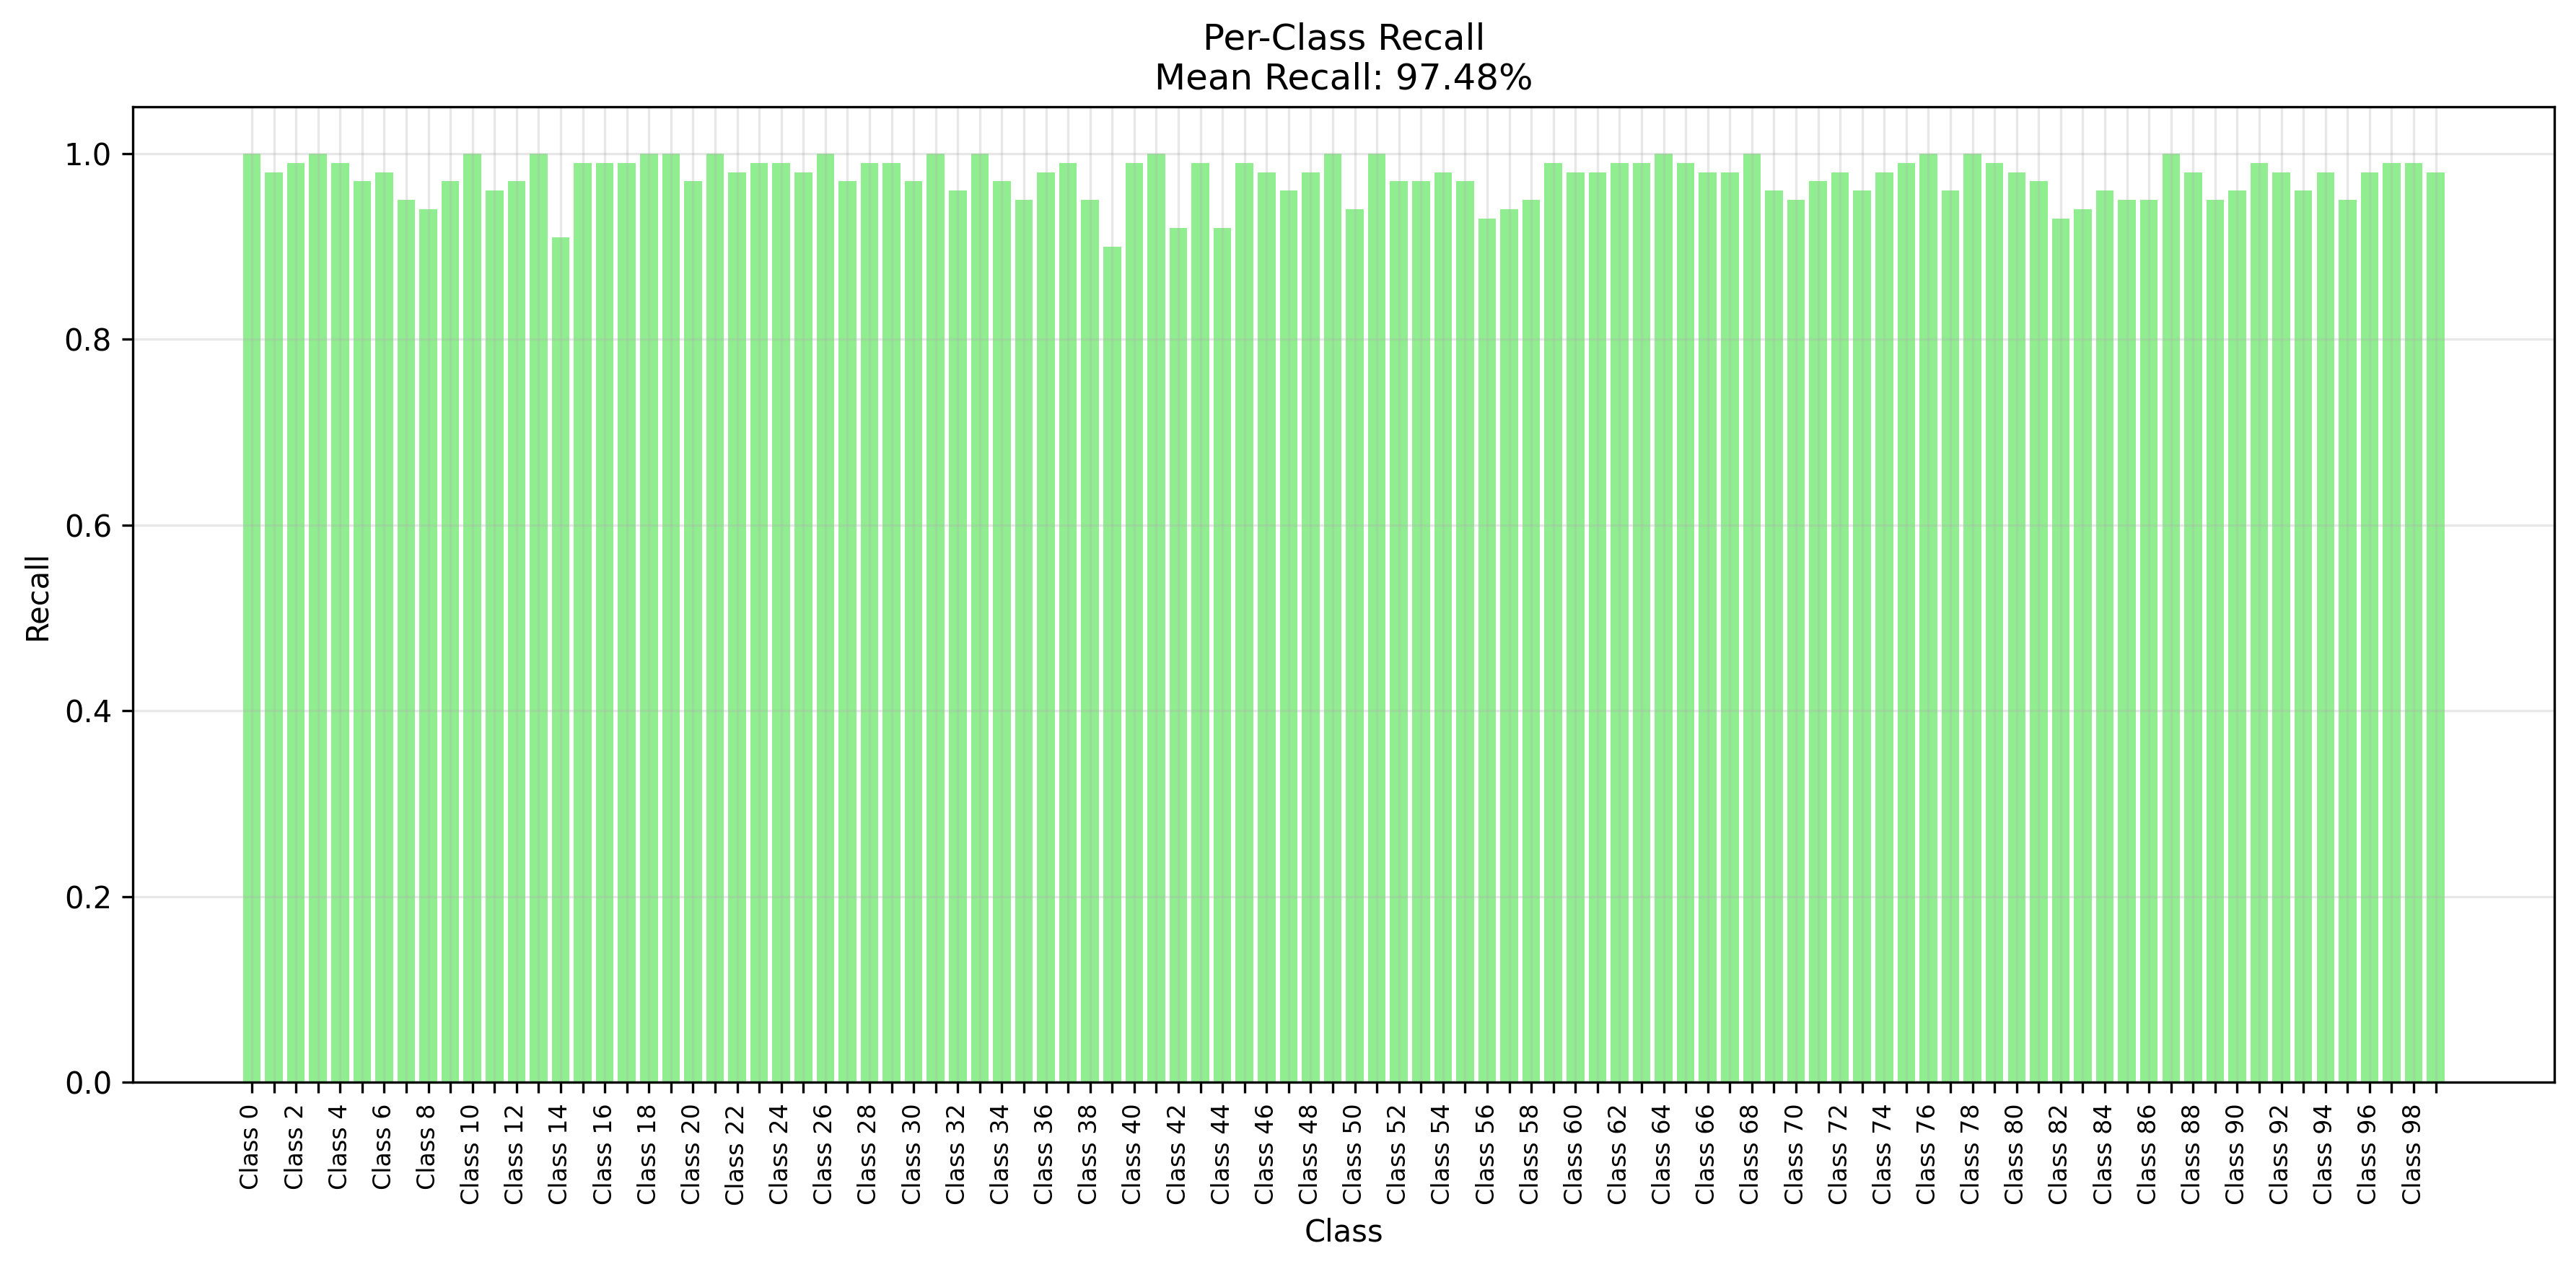
\includegraphics[width=\textwidth]{images/File3_final_analysis_recall.png}
        \caption{Per-class recall analysis}
        \label{fig:final_recall}
    \end{subfigure}
    \caption{Final model performance analysis on File3 dataset showing per-class metrics}
    \label{fig:final_analysis}
\end{figure}

\section{Detection}

\subsection{Detection Methodology}

\begin{figure}[h]
  \centering
  \begin{subfigure}[b]{0.2\textwidth}
      \centering
      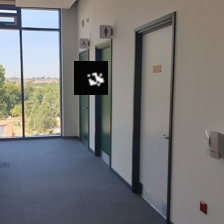
\includegraphics[width=\textwidth]{images/aruco-file4-detection-1.png}
      \caption{Marker in office placement example 1}
      \label{fig:det_ex_1}
  \end{subfigure}
  \hfill
  \begin{subfigure}[b]{0.2\textwidth}
      \centering
      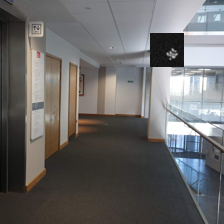
\includegraphics[width=\textwidth]{images/aruco-file4-detection-2.png}
      \caption{Marker in office placement example 2}
      \label{fig:det_ex_2}
  \end{subfigure}
  
  \vspace{0.5cm}
  
  \begin{subfigure}[b]{0.2\textwidth}
      \centering
      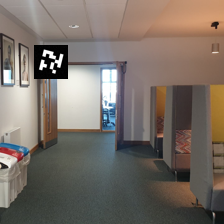
\includegraphics[width=\textwidth]{images/aruco-file4-detection-3.png}
      \caption{Marker in office placement example 3}
      \label{fig:det_ex_3}
  \end{subfigure}
  \hfill
  \begin{subfigure}[b]{0.2\textwidth}
      \centering
      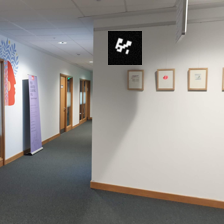
\includegraphics[width=\textwidth]{images/aruco-file4-detection-4.png}
      \caption{Marker in office placement example 4}
      \label{fig:det_ex_4}
  \end{subfigure}
  \caption{Examples of ArUco marker placements (from the provided dataset)}
  \label{fig:detection_examples}
\end{figure}

Figure \ref{fig:detection_examples} shows detection dataset examples. One hundred ArUco placements are included, alongside 
a CSV listing each marker's position.

The detection problem was approached similarly to classification with these steps: 

\begin{enumerate}
  \item The data plotter was adapted for detection data and results.
  \item A data augmentation script was created for office images with ArUco markers.
  \item Detection network architectures were prepared.
  \item An experiment was designed to compare detection architectures and settings.
  \item The final detection model was trained and tested.
\end{enumerate}

\subsubsection{Data Preparation}

Firstly, the dataset browser was adapted for detection data viewing and results. It displays the image, bounding box, pixel
distribution, and basic dataset statistics. This is visible in Figure \ref{fig:data_browser_2}.

\begin{figure}[h]
  \centering
  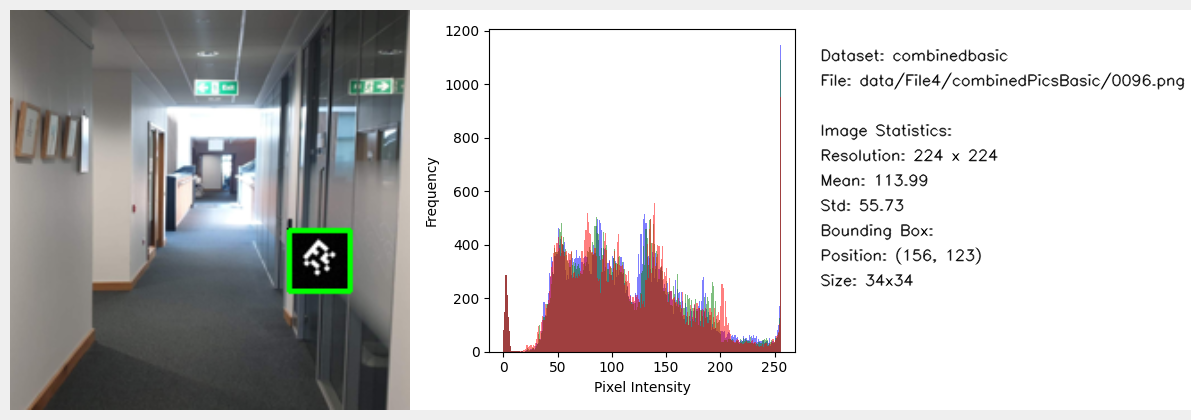
\includegraphics[width=0.45\textwidth]{images/aruco-dataset-browser-2.png}
  \caption{Dataset browser used with the File4 dataset}
  \label{fig:data_browser_2}
\end{figure}

After the data were analysed, a data augmentation script was developed to expand the training dataset, as the provided one was
insufficient compared to classification. The data browser was used to identify an optimal approach.

The data augmentation pipeline is outlined below:

\begin{figure}[H]
\begin{algorithm}[H]
\caption{Detection Data Preparation Pipeline}
\begin{algorithmic}[1]
\STATE Load office images and ArUco tags
\FOR{each office image}
    \STATE Get random 1000x1000 crop from original image
    \STATE Resize cropped image to 224x224
    \FOR{each ArUco class}
        \STATE Select random tag from custom dataset 1
        \STATE Resize tag to 34x34
        \STATE Calculate valid random position
        \STATE Place tag at position
        \STATE Save combined image
        \STATE Store bounding box coordinates
    \ENDFOR
\ENDFOR
\STATE Save bounding box annotations to CSV
\end{algorithmic}
\end{algorithm}
\caption{Detection data preparation workflow}
\end{figure}

\subsubsection{Network Architectures}

Multiple pre-trained PyTorch architectures were implemented. RetinaNet and MobileNet worked out of the box, whereas others were
problematic (YOLOv3) and later abandoned. Final models were based on \textcite{pytorch_retinanet}, \textcite{pytorch_fasterrcnn},
and \textcite{pytorch_mobilenet_rcnn}, chosen for performance and easy implementation.

\begin{itemize}
    \item \textbf{RetinaNet with ResNet50 backbone}: $\sim$40M parameters
    \begin{itemize}
        \item Pre-trained on ImageNet dataset for general object recognition (\cite{pytorch_retinanet})
    \end{itemize}
    
    \item \textbf{Faster R-CNN with ResNet50 backbone}: $\sim$38M parameters
    \begin{itemize}
        \item Pre-trained on ImageNet dataset for general object recognition
        \item Two-step detection: first finds regions of interest, then classifies them (\cite{pytorch_fasterrcnn})
    \end{itemize}
    
    \item \textbf{MobileNetV3-Large with FPN}: $\sim$20M parameters
    \begin{itemize}
        \item Pre-trained on ImageNet dataset for general object recognition
        \item Originally optimised for mobile/edge devices with fewer parameters (\cite{pytorch_mobilenet_rcnn})
    \end{itemize}
\end{itemize}

\subsubsection{Training Configuration}

Similarly to classification, the detection training pipeline included:

\begin{itemize}
  \item \textbf{Datasets}: File5 (provided dataset with 100 images of the office with tags with strong distortions to test the detection models)
  \item \textbf{Models}: RetinaNet-ResNet50, FasterRCNN-ResNet50, MobileNetV3-Large-FPN
  \item \textbf{Batch Sizes}: 4
  \item \textbf{Additional Random Training Transformations}: None, this is not to distort the office images, since the tags are already distorted
\end{itemize}

Only three distinct networks and result sets were produced. With one configuration file change, the entire experiment can be altered:
the custom dataset can be included (increasing epoch time), different batch sizes can be used (potentially exceeding GPU memory), and
varied models can be tested.

Additional settings and parameters were used solely to reduce experiment runtime:

\begin{itemize}
    \item \textbf{Optimizer}: Adam with learning rate 3e-4
    \item \textbf{Training Duration}: 100 epochs with early stopping at 98\% training accuracy 
\end{itemize}

After the experiments, results were plotted and analysed. They are presented in the following section, with full results in the results
directory and appendices.

The final model was trained on the custom dataset using parameters and settings derived from the best-performing initial experiments:

\begin{itemize}
  \item Batch size of 8 (GPU memory constrained)
  \item 50 training epochs
  \item Early stopping at 99.6\% IoU threshold
  \item Separate evaluation on File4 and File5
\end{itemize}

The implementation is identical to the classification approach. The Intersection over Union (IoU) metric was used to track progress, as
it measures bounding box overlap. Only one bounding box and one class exist per image; mean IoU and mean Mean Absolute Error (MAE) were
used for evaluation.

\subsection{Detection Results}

Detection experiments were conducted in two phases, mirroring the classification procedure. Multiple architectures were tested on File5
to determine the optimal approach. The best-performing configuration was then trained on a custom dataset and evaluated against both File4 and File5.

\subsubsection{Initial Experiments}

The selected architectures were used with a batch size of four due to GPU memory constraints. Each configuration was tested on 1000 samples
from File5, outputting the following results:

\begin{itemize}
  \item \textbf{FasterRCNN-ResNet50}:
    \begin{itemize}
        \item Batch size 4: Mean IoU: 97.80\%
    \end{itemize}
    
  \item \textbf{MobileNetV3-Large-FPN}:
    \begin{itemize}
        \item Batch size 4: Mean IoU: 95.93\% 
    \end{itemize}

  \item \textbf{RetinaNet-ResNet50}:
    \begin{itemize}
        \item Batch size 4: Mean IoU: 98.05\%
    \end{itemize}
\end{itemize}

The results are shown in Figure \ref{fig:training_progress_detection}.

\begin{figure}[h]
    \centering
    \begin{subfigure}[b]{0.45\textwidth}
      \centering
      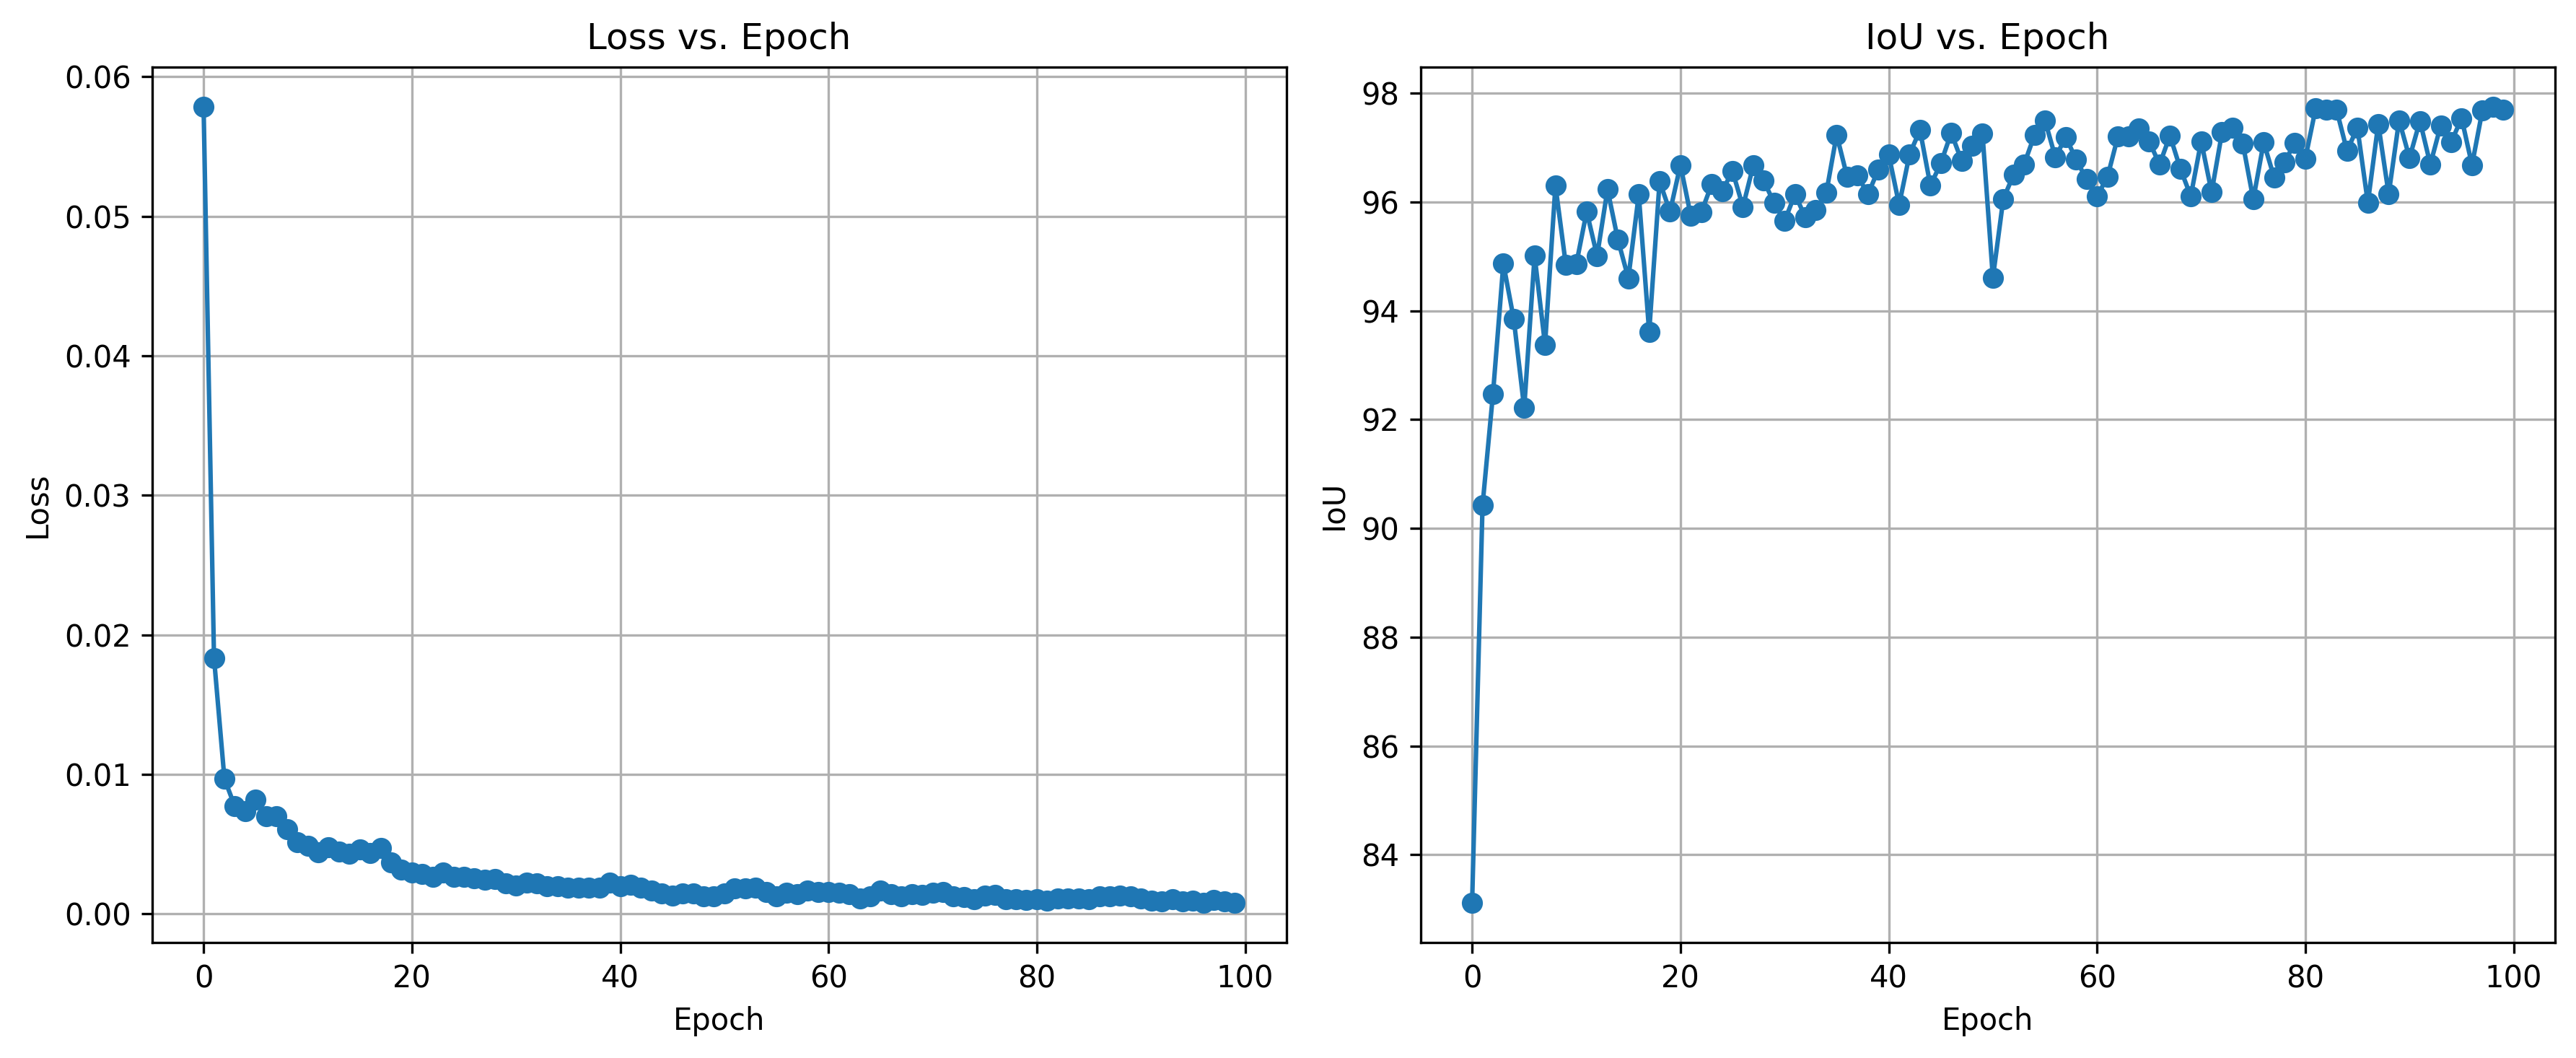
\includegraphics[width=\textwidth]{images/File5_FasterRCNN_training_progress.png}
      \caption{FasterRCNN training progress}
      \label{fig:progress_fasterrcnn}
    \end{subfigure}
    \hfill
    \begin{subfigure}[b]{0.45\textwidth}
      \centering
      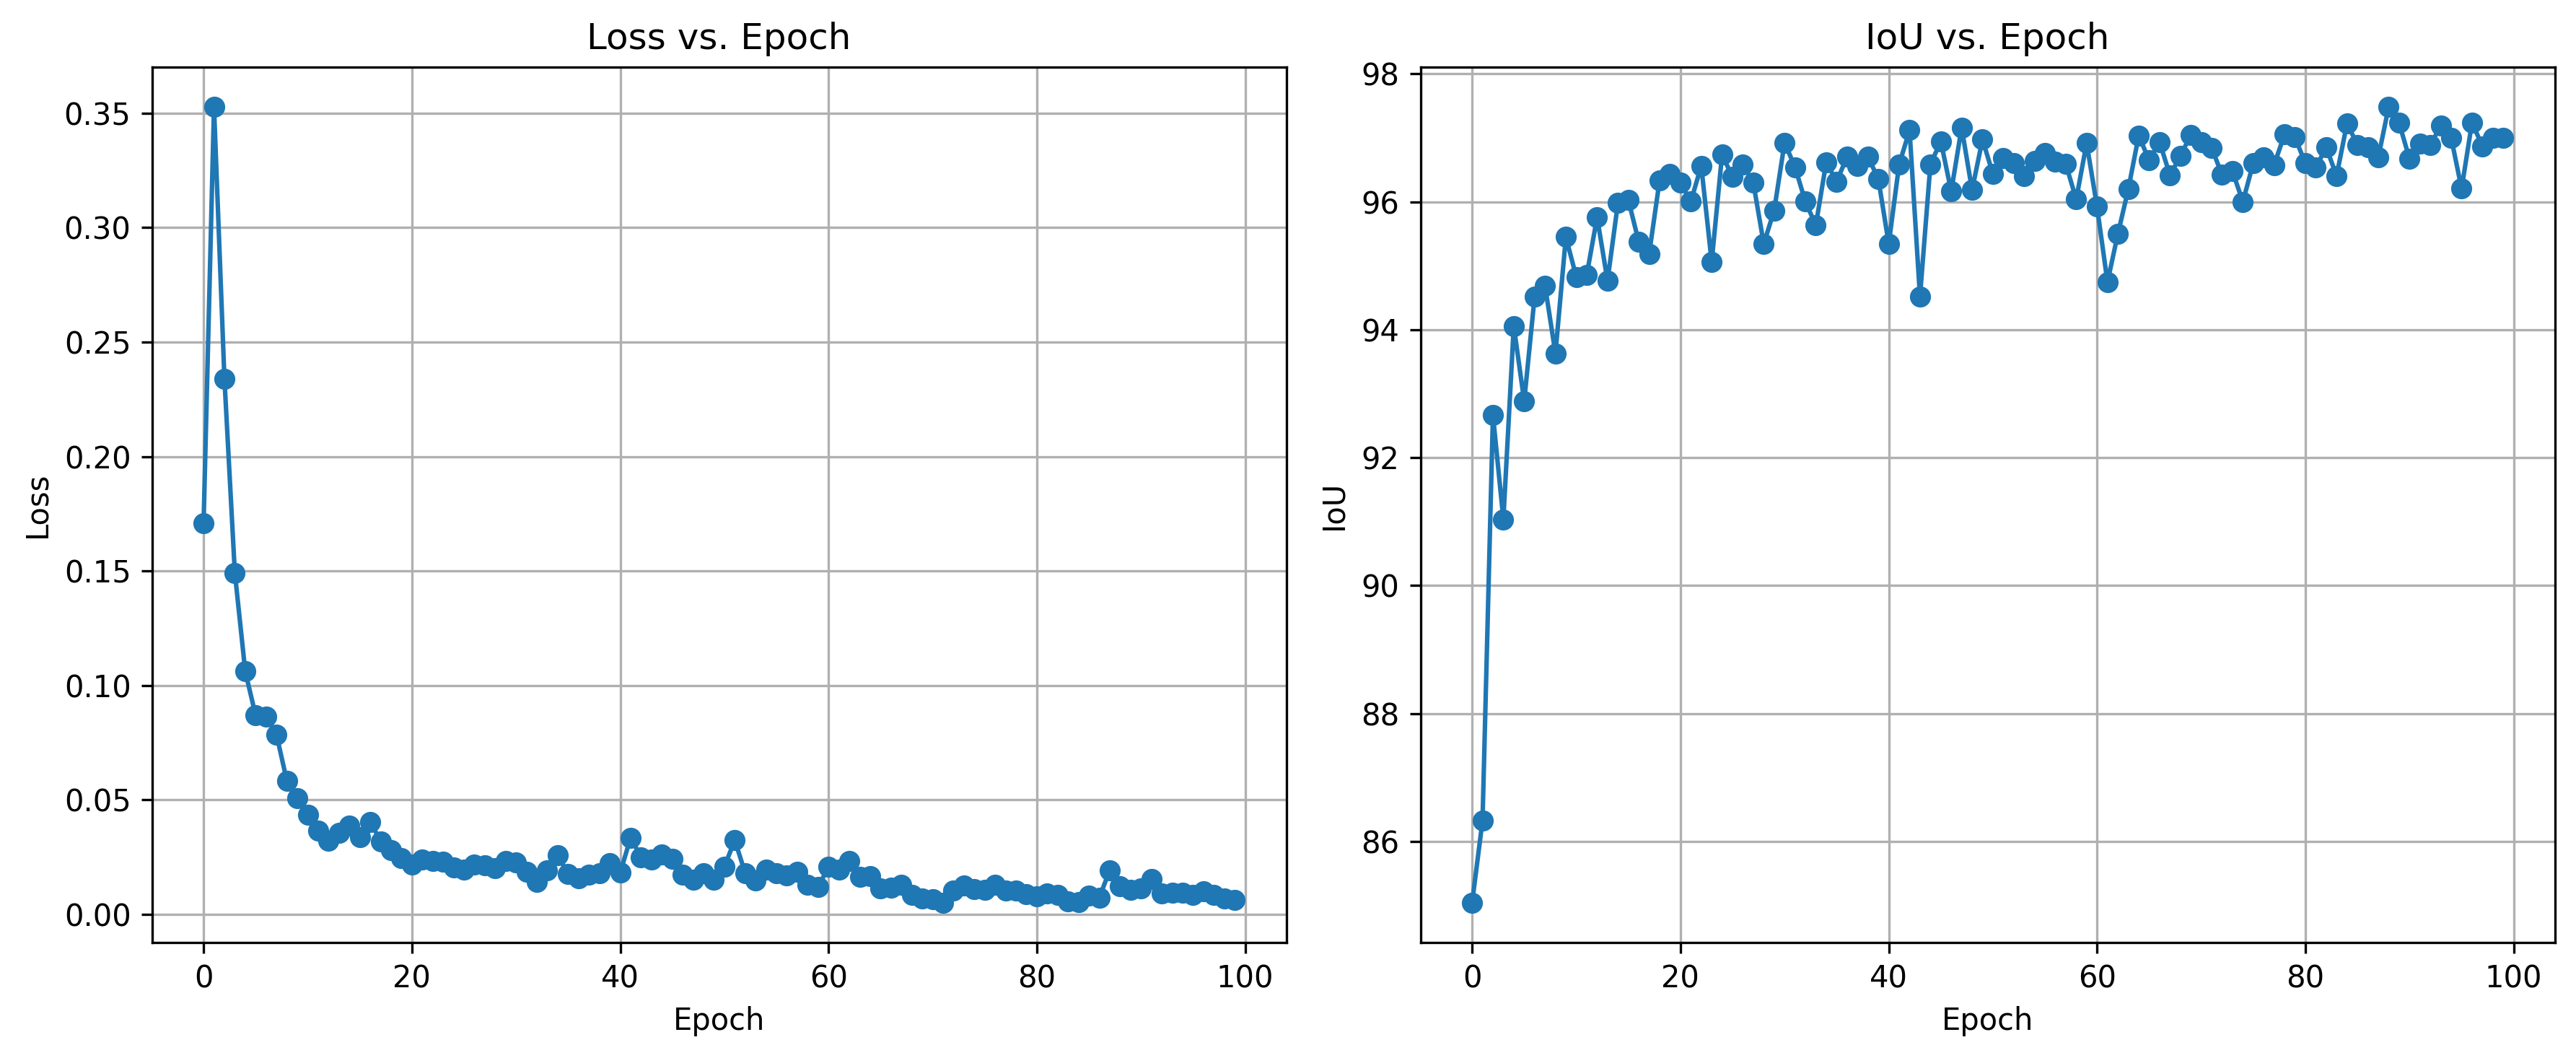
\includegraphics[width=\textwidth]{images/File5_MobileNet_training_progress copy.png}
      \caption{MobileNet (pre-trained) training progress}
      \label{fig:progress_mobilenet}
    \end{subfigure}    
    \vspace{0.5cm}
    \begin{subfigure}[b]{0.45\textwidth}
      \centering
      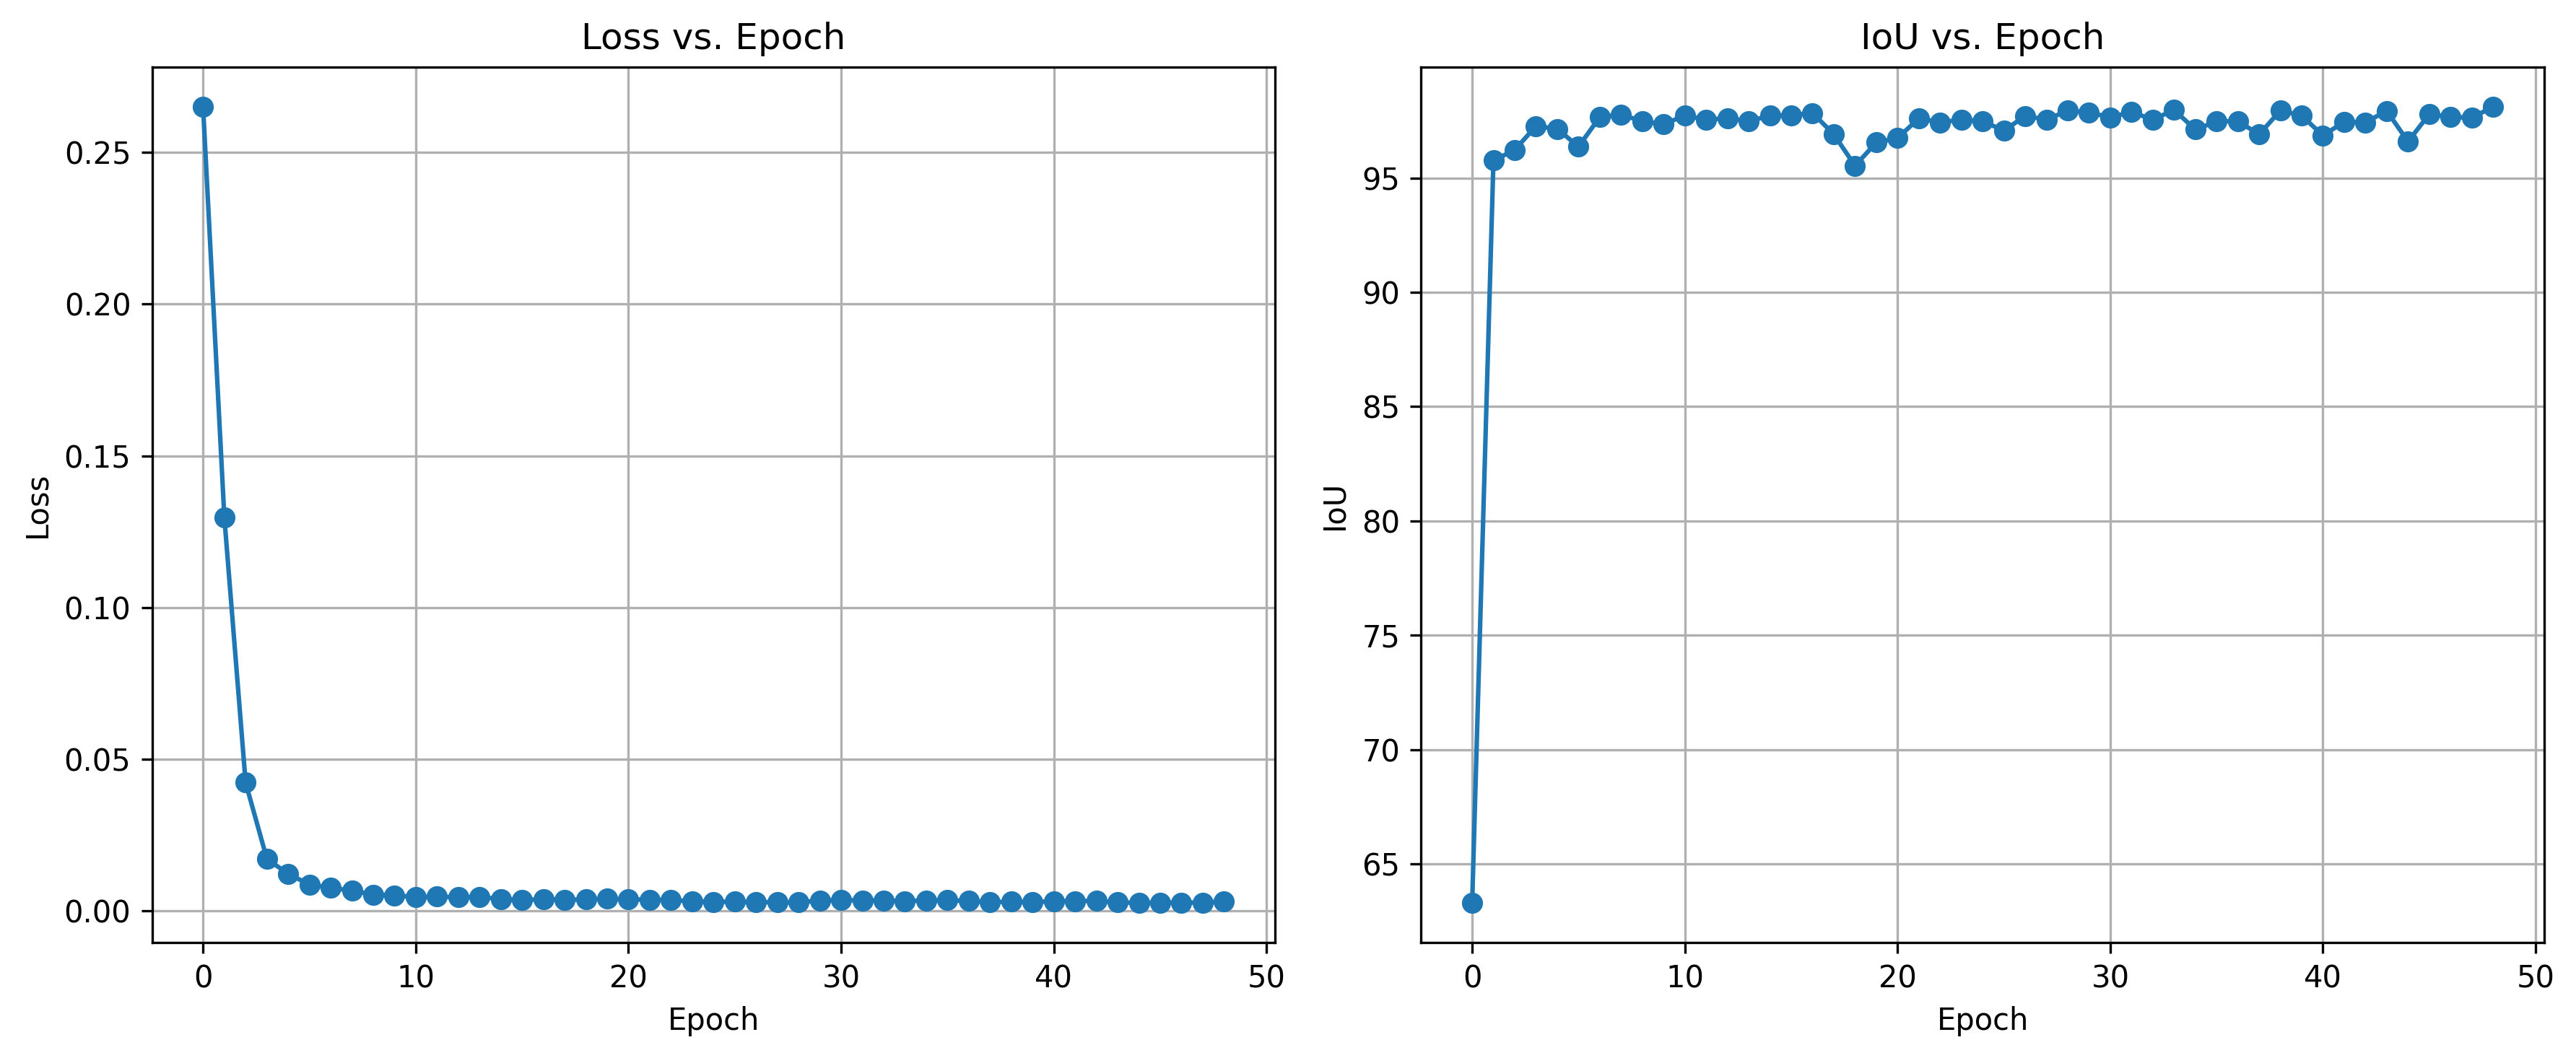
\includegraphics[width=\textwidth]{images/File5_RetinaNet_training_progress.png}
      \caption{RetinaNet (pre-trained) training progress}
      \label{fig:progress_retinanet}
    \end{subfigure}
    \caption{Training progress for different model architectures showing training loss and IoU over epochs}
    \label{fig:training_progress_detection}
\end{figure}

The RetinaNet model was observed to perform the best and converge the fastest, exhibiting the highest IoU and lowest loss.

\subsubsection{Final Model Performance}

RetinaNet with a ResNet50 backbone was selected as the final model due to its performance. It was trained on FileCustom2, a 
synthetic dataset approximating conditions in Files 4 and 5. A set of 10,000 images was used, but this is adjustable in the configuration 
file. This was done to conserve time and resources, as the dataset was large enough, and augmentation plus each epoch were lengthy.

The final evaluation produced these results:

\begin{itemize}
    \item \textbf{Training Evaluation} (1,000 testing samples):
        \begin{itemize}
            \item Mean IoU: 99.70\%
        \end{itemize}
    \item \textbf{File4 Evaluation} (100 of the provided samples):
        \begin{itemize}
            \item Mean IoU: 89.00\%
        \end{itemize}
    \item \textbf{File5 Evaluation} (100 of the provided samples):
        \begin{itemize}
            \item Mean IoU: 85.64\%
        \end{itemize}
\end{itemize}

Strong performance was demonstrated across various distortion conditions. A perfect detection rate on File4 (IoUs over 50\%) indicated 
effective handling of weak distortions. On File5, only three out of 100 markers were missed, showing resilience to more demanding conditions. 
The missed markers (and other results) can be seen in Figure \ref{fig:final_detection_examples}.

\begin{figure}[h]
  \centering
  \begin{subfigure}[b]{0.45\textwidth}
    \centering
    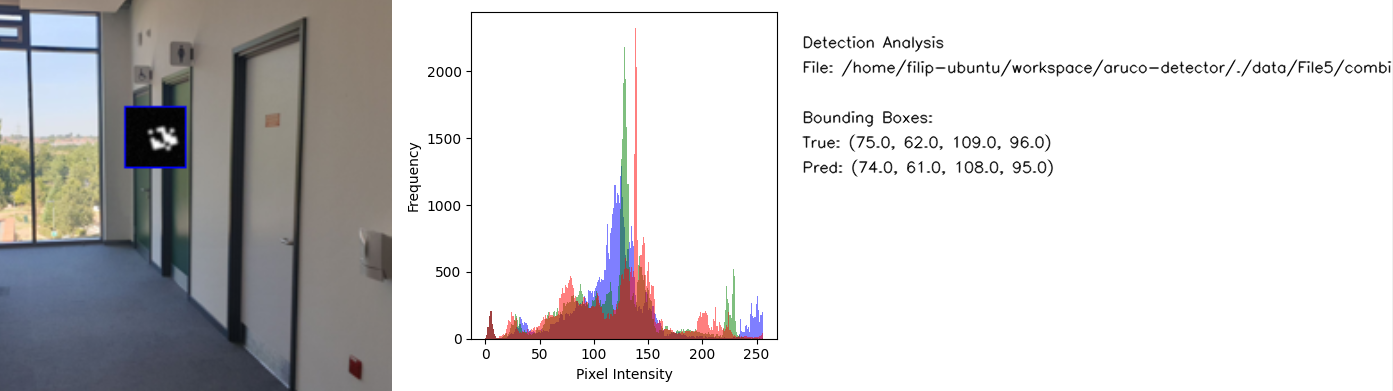
\includegraphics[width=\textwidth]{images/result_vis_1.png}
    \caption{Example 1}
    \label{fig:det_res_ex1}
  \end{subfigure}
  \hfill
  \begin{subfigure}[b]{0.45\textwidth}
    \centering
    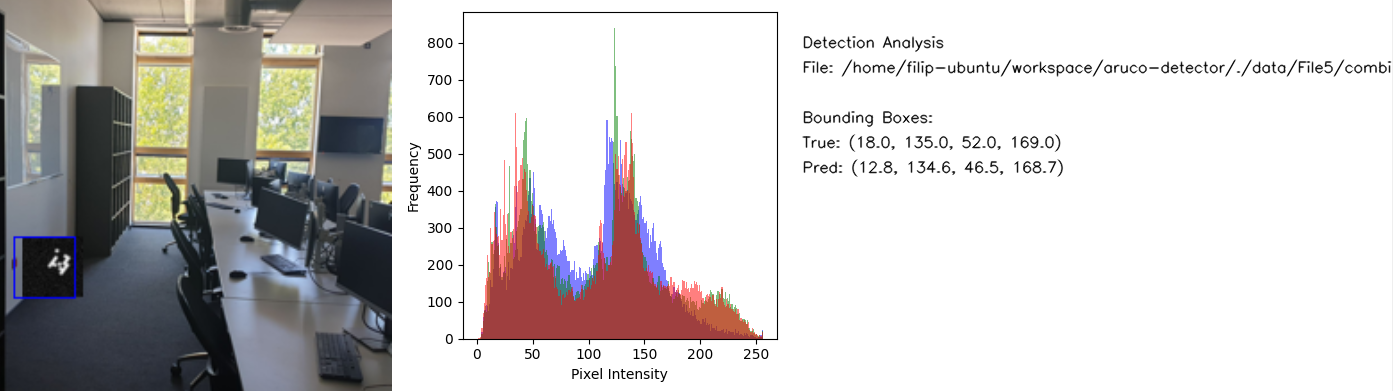
\includegraphics[width=\textwidth]{images/result_vis_2.png}
    \caption{Example 2}
    \label{fig:det_res_ex2}
  \end{subfigure}    
  \vspace{0.5cm}
  \begin{subfigure}[b]{0.45\textwidth}
    \centering
    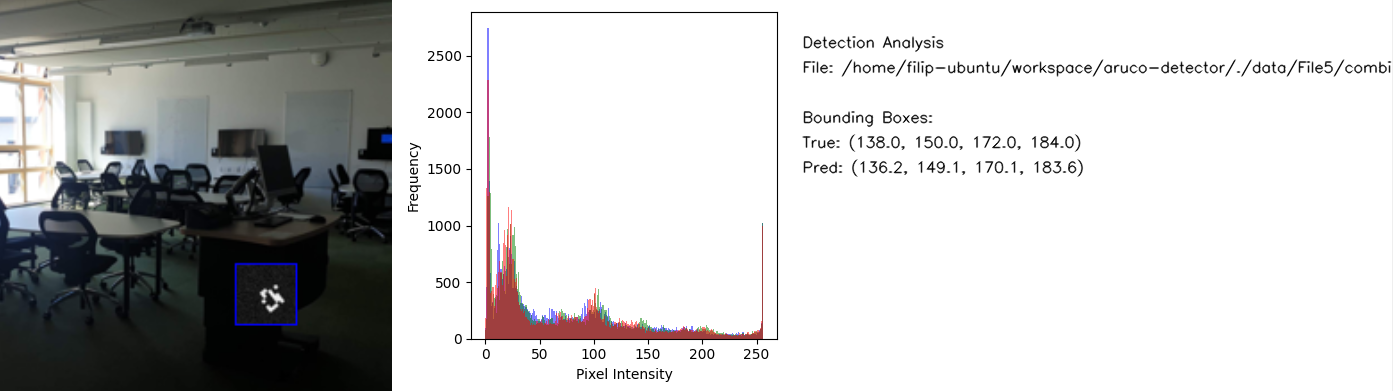
\includegraphics[width=\textwidth]{images/result_vis_4.png}
    \caption{Example 3}
    \label{fig:det_res_ex3}
  \end{subfigure}
  \hfill
  \begin{subfigure}[b]{0.45\textwidth}
      \centering
      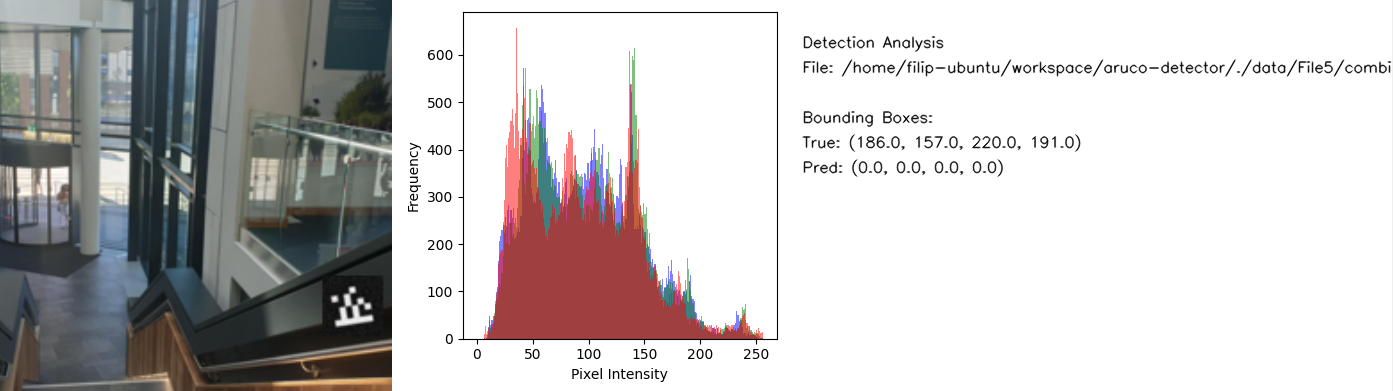
\includegraphics[width=\textwidth]{images/result_vis_5.png}
      \caption{Example 4}
      \label{fig:det_res_ex4}
  \end{subfigure}
  \caption{Final detection model prediction examples}
  \label{fig:final_detection_examples}
\end{figure}

\section{Conclusion}

Deep learning approaches for ArUco marker detection and classification under challenging conditions were explored. Several key findings emerged:

\begin{itemize}
    \item \textbf{Classification Performance}: GoogLeNet was observed to achieve near-perfect accuracy (100\%) on weakly distorted markers
    and to maintain robust performance (97.48\%) even under severe distortions, thereby confirming that transfer learning is effective.
    The custom model was found to perform better after extended training, as verified individually in the GitHub commit d9fd8ad.
    
    \item \textbf{Detection Performance}: Excellent performance in localising markers was shown by RetinaNet with ResNet50 backbone, achieving
    89.00\% IoU in basic office scenarios and 85.64\% IoU under challenging conditions. Occasional (0,0) predictions highlighted the need 
    for longer training.
    
    \item \textbf{Architecture Insights}: Pre-trained models consistently outperformed custom architectures.
    
    \item \textbf{Technical Limitations}: GPU memory constraints restricted batch sizes and training duration, with each detection-model
    epoch requiring 20 minutes at the current state. With greater compute, the batch size should be increased and the dataset expanded
    through the configuration file to improve detection outcomes. More settings and parameters could then easily be tested and compared.

    \item \textbf{Augmentation Mistake}: Additional data augmentation on pre-augmented images proved counterproductive for the reason
    that the images were already augmented.
\end{itemize}

Future improvements that could yield interesting results include: 

\begin{itemize}
    \item Expanding synthetic dataset generation with perspective transformations, partial occlusion, and other distortions
    \item Implementing larger batch sizes and extended training (more compute required)
    \item Collecting real-world data to validate synthetic training results
    \item Testing more pre-trained detection models given sufficient computational resources
\end{itemize}

These outcomes show the viability of deep learning for marker detection, although systematic improvements, resource expansion,
and thorough validation remain highly essential.

\printbibsection

\appendices

\renewcommand{\thesection}{\Alph{section}}

\section{GitHub Repository}

The GitHub repository for this project can be found at the following link: \url{https://github.com/FHanus/aruco-detector}.

The repository contains the following key components that should be viewed in order to more thoroughly understand the project:

\begin{enumerate}
    \item \textbf{Results, classification, per trained model:}
    \begin{itemize}
        \item Per class accuracy plots
        \item Per class confusion matrices
        \item Per class precision plots
        \item Per class recall plots
        \item Training progress plots
        \item CSVs with evaluation predictions and data
    \end{itemize}

    \item \textbf{Results, detection, per trained model:}
    \begin{itemize}
        \item IoU distribution plots
        \item Training progress plots
        \item CSVs with evaluation predictions and data
    \end{itemize}

    \item \textbf{Data:}
    \begin{itemize}
        \item Original datasets (File1-File5)
        \item Custom synthetic datasets (Custom1-Custom2)
    \end{itemize}

    \item \textbf{Docs:}
    \begin{itemize}
        \item This LaTeX paper
        \item README explaining the repository more thoroughly
        \item Training log file
    \end{itemize}

    \item \textbf{Scripts:}
    \begin{itemize}
        \item All of the code
    \end{itemize}
\end{enumerate}

This repository represents a complete research project on ArUco marker detection and classification, including code
implementation, experimental results, and detailed documentation.

\end{document}